% !TeX program = xelatex
% 2026 CUMCM 电子版论文示例：电子版第一页必须是摘要专用页。
% 编译：latexmk -xelatex cumcm.tex
\documentclass[zihao=-4,a4paper,UTF8,fontset=none]{ctexart}

% template
\input{cumcm-latex-template-2026/cumcm2026.sty}

% set English and Number font
\setmainfont{TimesNewRoman.ttf}[
  Path=cumcm-latex-template-2026/fonts/,
  BoldFont=TimesNewRomanBold.ttf,
  ItalicFont=TimesNewRomanItalic.ttf,
  BoldItalicFont=TimesNewRomanBoldItalic.ttf
]



% set Chinese font
\setCJKmainfont[
  Path=cumcm-latex-template-2026/fonts/,
  BoldFont=SimHei.ttf
]{SimSun.ttc}

\setCJKfamilyfont{zhsong}[
  Path=cumcm-latex-template-2026/fonts/
]{SimSun.ttc}

\setCJKfamilyfont{zhhei}[
  Path=cumcm-latex-template-2026/fonts/,
  BoldFont=SimHei.ttf
]{SimHei.ttf}
\setCJKmonofont[
  Path=cumcm-latex-template-2026/fonts/
]{SimSun.ttc}

\providecommand{\songti}{}
\providecommand{\heiti}{}
\renewcommand{\songti}{\CJKfamily{zhsong}}
\renewcommand{\heiti}{\CJKfamily{zhhei}}






% 本地论文排版：沿用 cumcm2026.sty，正文与摘要由同目录文件载入。
% 修改论文结构与文字请编辑 docs/论文正文.md，再运行 ../paper_structure_review/build_paper.py。
\usepackage{etoolbox}
\titleformat{\section}{\centering\heiti\zihao{4}}{\chinese{section}、}{0.3em}{}
\titleformat{\subsection}{\heiti\zihao{-4}}{\thesubsection}{0.7em}{}
\titleformat{\subsubsection}{\heiti\zihao{-4}}{\thesubsubsection}{0.7em}{}
\linespread{1.15}
\setlength{\emergencystretch}{2em}
\setlength{\parskip}{0pt}
\widowpenalty=10000
\clubpenalty=10000
\setcounter{secnumdepth}{3}
% 供无编号 longtable 使用；Pandoc 将其类型标记为 none。
\newcounter{none}
\providecommand{\tightlist}{\setlength{\itemsep}{0pt}\setlength{\parskip}{0pt}}
\AtBeginEnvironment{longtable}{\small}
\renewcommand{\arraystretch}{1.22}
\setlength{\tabcolsep}{5pt}
\captionsetup{font=small,labelfont=normalfont,labelsep=quad}
\makeatletter
\renewcommand{\maketitle}{%
  \thispagestyle{plain}\setcounter{page}{1}%
  \begin{center}
    {\heiti\zihao{3}\@title\par}
    \vspace{1em}
    {\heiti\zihao{4}摘\quad 要\par}
  \end{center}}
\makeatother
\title{基于联合残差情景与动态价值调度的微网购电优化}
\begin{document}
\maketitle
\begin{cumcmabstract}
\linespread{1.02}\selectfont
% 强制摘要首段按中文排版首行缩进两字；后续自然段由空行自动缩进。
\par\indent% ===== 摘要正文（由论文正文.md生成）=====
针对\textbf{光伏储能}小区中购电计划须提前申报而实际供需持续变化的矛盾，本文研究\textbf{计划购电}、\textbf{紧急补购}与\textbf{储能库存}的协同配置。基于供需平衡、储能容量、充放电功率、转换效率及动作互斥等约束，依次建立确定性联合优化、历史情景规划和多时点滚动调整模型，并以\textbf{动态规划}构造未来近似成本函数，权衡当前购电成本与储能的远期机会价值。

\textbf{针对问题一，}建立\textbf{确定性购电---储能联合优化模型}。以分时电价下的购电成本最小化为目标，利用储能状态递推关联各时段决策，并将日首、日末储电量均约束为6000 kWh；在此基础上同步优化计划购电量及储能充放电量，实现净负荷消纳与跨时段能量转移。结果显示，最小费用方案的单日购电量为59.483 MWh，购电成本为3.513万元。

\textbf{针对问题二，}建立\textbf{联合残差情景规划与动态价值调度模型}。模型按历史日期匹配负荷与光伏预测残差，以保留源荷误差的相关性和日内时序特征；日前层构建\textbf{情景混合整数线性规划（MILP）}，以全网统一购电计划为决策变量，最小化计划购电成本与期望紧急补购成本，并采用1月标定期参数设置终端库存价值；实时层借助\textbf{历史情景动态规划}近似未来成本，权衡当期补购支出与库存机会成本。334天回放结果表明，该方案总费用为1376.393万元，较贪心调度方案减少10.666万元，降幅为0.769\%。两组方案期末库存一致；尽管所提方案的紧急购电量由172.161 MWh增至176.902 MWh，其加权平均补购单价却由5.942元/kWh降至5.181元/kWh，表明费用改善主要来自补购时点与储能库存的协同配置。

\textbf{针对问题三，}建立\textbf{光伏预报更新驱动的多时点滚动优化模型}。模型利用每日0:00、6:00、12:00和18:00发布的光伏预报，在锁定已执行时段决策的前提下动态修正剩余时段的购电计划；分段线性调整结算费用、期望紧急补购费用和终端库存价值共同构成优化目标，并同步更新\textbf{动态规划近似价值函数}。在相同的334天评价期内，允许日内调整方案的总费用为1326.878万元，较无调整方案减少62.894万元，降幅为4.525\%；紧急购电量由180.018 MWh降至29.540 MWh，降幅为83.590\%。两项指标均表明，利用日内新预报调整未执行计划是必要的。

\textbf{针对问题四，}考虑电价波动且未来价格不可预知的运行环境，建立\textbf{因果价格预测下的源荷情景调度模型}。模型利用此前已实现的价格形成未来价格点预测，并在该预测价格下构造负载---光伏联合残差情景，据此重新求解日前锁定调度和多时点滚动优化方案。334天波动电价回放结果显示，日前方案和滚动优化方案的总费用分别为1454.019万元和1415.219万元，后者减少38.800万元，降幅为2.668\%；紧急购电量由181.144 MWh降至59.464 MWh，降幅为67.17\%。由于情景规模、光伏信息和更新机制也不同，该结果属于综合方案差异，不能完全归因于日内调整，也不与固定分时电价结果直接比较。进一步的同信息条件独立闭环消融表明，单独开放日内计划调整权限可使全年费用降低3.973\%，紧急购电量减少65.715\%。

研究结果表明，储能的经济价值不仅体现在削减紧急补购量，更体现在优化补购时序并保障高价时段的供能能力；\textbf{历史情景规划}可将预测误差前置纳入日前决策，\textbf{日内滚动优化}则可利用实时预报修正计划。在能够获取日内更新预报并支持购电计划动态调整的场景中，滚动优化结合动态价值调度的方案表现更优。

\cumcmkeywords{光伏储能调度；混合整数线性规划；情景随机规划；联合残差场景；滚动时域优化；动态规划；近似价值函数}
\end{cumcmabstract}
% ===== 论文正文（由论文正文.md生成）=====
\section{问题重述}\label{ux95eeux9898ux91cdux8ff0}

\subsection{问题背景}\label{ux95eeux9898ux80ccux666f}

本文研究的小区微网由小区负载、光伏发电单元、储能装置和外部电网组成。光伏出力与负载需求存在时序错配，储能可通过跨时段充放电缓解源荷不平衡，但其运行受额定容量、充放电功率、转换效率和安全储电范围等物理约束。此类``预测---计划---实时执行''的分层调度是微网能量管理的常见结构{[}1{]}。当计划购电、实际光伏出力和储能放电仍不足以满足负载时，系统通过紧急购电补足缺额，紧急购电单价按对应槽位电价的5倍计算。基于上述机制，本文针对不同信息条件和电价环境，依次优化日前购电计划、日内滚动购电调整及储能实时充放电策略，在保证供需平衡和储能安全运行的前提下控制实际购电费用。

本文将每日24 h划分为144个10分钟槽，单槽时长为 \(\Delta t=1/6\ \mathrm h\)。储能额定容量为12000 kWh，安全储电范围为1200～10800 kWh，最大充、放电功率均为5000 kW，充、放电效率均为90\%。整个年度仿真以2025年1月1日0:00的储电量6000 kWh为初始状态；除问题一按照题目要求设置单日首末储电量约束外，问题二至问题四的实际SOC均在相邻时段和相邻日期之间连续传递，不进行每日重置。

\subsection{问题提出}\label{ux95eeux9898ux63d0ux51fa}

题目将每个自然日划分为144个10分钟时段，要求结合附件1至附件4提供的分时电价、实际负载、实际光伏、光伏预报及波动电价数据，制定购电计划与储能充放电策略。四个问题采用相同的储能物理参数，但数据范围、信息可用条件和购电调整机制逐步扩展。

\textbf{·问题一：} 附件1给出了典型日各时段的小区负载、光伏预测功率和分时电价。要求建立单日购电与储能联合优化模型，在满足日初与日末储电量相等的条件下，给出指定时段的计划购电量、全天计划购电量及费用，并统计储能充放电结果。

\textbf{·问题二：} 分时电价曲线每日相同，而小区负载和光伏实际功率随日期及时段变化。要求每天0:00制定当日计划购电策略。当计划购电、光伏出力及储能放电仍不足以满足负载时，按对应交易时刻正常电价的5倍进行紧急购电。需要给出指定日期的计划购电量、储能充放电量、紧急购电量及相关费用，并将完整策略写入指定结果文件。

\textbf{·问题三：} 每天0:00、6:00、12:00和18:00可获得未来24小时的光伏功率预报。0:00预报用于制定当日原始购电计划，其余时点的新预报可用于调整尚未执行的购电安排。对于购电下调部分，违约电价为交易时刻电价的50\%；对于超过原计划的上调部分，超出电量按交易时刻电价的150\%计费。要求建立多时点滚动购电模型，给出指定日期的调度结果，并分析是否有必要利用6:00、12:00和18:00发布的新预报调整购电策略。

\textbf{·问题四：} 外部电网电价随日期及时段实时波动。要求利用附件4的波动电价，以及附件2、附件3中的实际源荷和光伏预报数据，分别在问题二和问题三的信息结构下重新制定购电策略，并将两类完整结果分别写入指定文件。

\section{问题分析}\label{ux95eeux9898ux5206ux6790}

\subsection{问题一的分析}\label{ux95eeux9898ux4e00ux7684ux5206ux6790}

问题一的关键在于协调购电与储能充放电。日首、日末储电量满足 \(E_0=E_{144}=6000\text{ kWh}\)，使不同方案能够在相同的储电量基准下比较；充放电效率 \(\eta_c,\eta_d\) 和单槽功率限制则决定电量跨时段转移的可行性与经济性。因此，各时段的购电量 \(p_t\) 不能独立确定，而需通过储能状态 \(E_t\) 的递推关系统一优化。本文以购电费用最小为目标建立确定性线性规划，并结合典型日运行轨迹分析购电与储能在不同时段的作用。

\subsection{问题二的分析}\label{ux95eeux9898ux4e8cux7684ux5206ux6790}

问题二需要在实际供需尚未实现时确定全天购电计划 \(p_{d,t}\)。计划偏小，实际净负荷高于预测值时可能触发5倍电价的紧急购电 \(e_{d,t}\)；计划偏大，则可能增加转换损耗或产生无法吸收的富余能量。为保留负载与光伏预测误差之间及其日内的相关结构，本文将同一历史日的两类残差 \((r^L_{j,t},r^G_{j,t})\) 整体抽取，构造源荷联合情景，并建立两阶段随机混合整数线性规划。日前购电量 \(p_{d,t}\) 在全部情景间共享，情景内的储能、弃能和紧急购电变量用于估计不同计划的补救代价。实际运行时，根据当前供需偏差、储电量 \(E_{d,t}\) 及近似未来成本 \(\overline H_t(E)\) 确定充放电动作，使日前计划与逐时响应相衔接。其中，未来成本由决策时已可得的历史情景近似构造，情景内的补救轨迹不直接作为实际调度指令。

\subsection{问题三的分析}\label{ux95eeux9898ux4e09ux7684ux5206ux6790}

日内新预报既可能改变储能的充放电安排，也为修正尚未执行的购电计划提供了依据。本文在0:00制定原计划 \(p_{d,t}\)。附件日内列以00:10、00:20、\ldots\ldots、24:00标记；按这一官方列序从0开始编号，0:00、6:00、12:00和18:00四个计划版本在冻结程序中分别从列索引 \(\rho_k\in\{0,35,71,107\}\) 开始生效。各次更新只使用已发布预报、已经完成的实测信息及当前SOC重新优化剩余计划；索引小于 \(\rho_k\) 的已执行列保持不变。调整时还需权衡修正供需偏差的收益与合同成本：上调量 \(\delta^+_{d,t}\) 按对应时段电价的150\%计费，下调量 \(\delta^-_{d,t}\) 承担50\%的违约成本。对于题目未明确的多次调整结算方式，本文约定每个时段仅依据最终生效量 \(z_{d,t}\) 与0:00原计划 \(p_{d,t}\) 的差异结算一次。评价时设置具有相同预报访问权限的禁止调整对照，考察开放购电调整的整体效果；另通过同计划、同初始SOC的配对消融分析储能执行规则的作用。

\subsection{问题四的分析}\label{ux95eeux9898ux56dbux7684ux5206ux6790}

问题四将固定分时电价替换为波动电价。在本文采用的``未来实际电价不可提前获知''假设下，购电决策需同时考虑供需偏差和价格预测误差 \(\pi^{\mathrm{act}}_{d,t}-\widehat\pi_{d,t}\)；电力市场不确定性下的决策问题可参见文献{[}2{]}。为此，模型仅利用决策时点前已经实现的实际电价计算未来价格点预测 \(\widehat\pi_{d,t}\)，并在该预测价格曲线下，以同一历史日的负载、光伏残差构造保留日内相关结构的源荷联合情景。价格残差用于开发期预测误差评价和代表日诊断，不作为正式MILP中的第三类情景维度。问题4-2采用日前计划锁定方案，问题4-3采用多时点滚动更新方案，实际价格 \(\pi^{\mathrm{act}}_{d,t}\) 仅用于当前时段执行与事后结算。比较时同时考察实际费用、紧急购电量及期末SOC，避免将库存差异误认为经济收益。由于两分支的情景规模、光伏信息和更新机制不同，其费用差反映两套综合方案的表现，不能全部归因于日内调整。

针对以上问题，本文采用以下整体思路框架进行系统性研究和分析。

\begin{figure}[H]
\centering
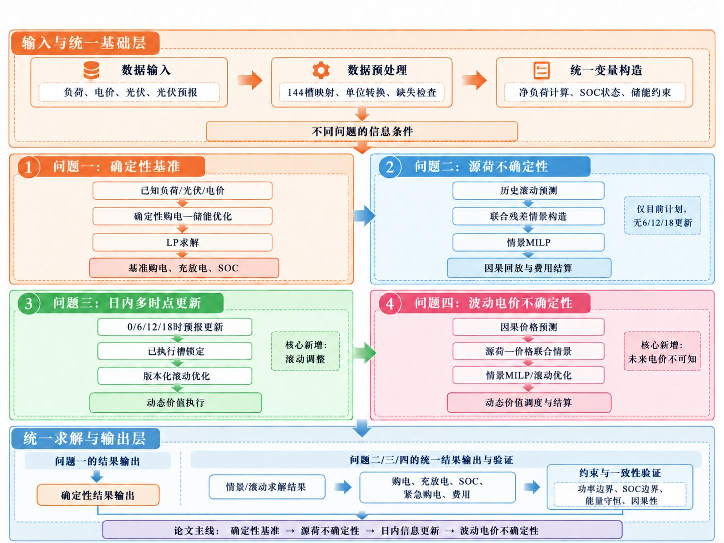
\includegraphics[width=.91\linewidth,height=.63\textheight,keepaspectratio]{../outputs/figures/paper_v2/overall_research_framework.pdf}
\renewcommand{\thefigure}{1-1}
\caption{整体思路框架}\label{fig:q1-1}
\end{figure}

\section{模型假设}\label{ux6a21ux578bux5047ux8bbe}

\begin{enumerate}
\def\labelenumi{\arabic{enumi}.}
\tightlist
\item
  \textbf{计量与时间假设：}以 10 min 为调度槽，槽内功率恒定，槽电量按功率×槽长换算；时间索引按附件原始行列映射，不作平移。
\item
  \textbf{储能与供能假设：}充、放电效率均取 0.9；充放电互斥；不向外部电网售电，超出可吸收能力的富余能量计为弃能；紧急购电仅用于补足实际供需缺口。
\item
  \textbf{信息边界假设：}日前或发布时点仅使用当时已可得信息，不预知未来实际值；实时层可观测当前槽供需并快速响应；历史残差仅由决策时点前已完整实现的数据构造。
\item
  \textbf{价格信息假设：}问题四中，当前槽实际价格在该槽开始时可得；计划阶段仅用此前已实现价格预测未来价格。
\item
  \textbf{调整结算假设：}问题三和 4-3 中，每槽最终生效量仅相对 0:00 原计划结算一次；上调部分按 1.5 倍对应槽电价计费，下调部分按对应槽电价的 50\% 计违约成本，紧急购电按 5 倍价格计费；中间版本不重复结算。
\item
  \textbf{预报时间映射假设：}附件3仅给出整点光伏预报时，采用相邻整点之间的分段线性插值生成10分钟槽预测；该处理只用于统一时间尺度，不额外引入未来实测信息。
\end{enumerate}

\textbf{约束说明：}日首/日末储电量、功率与安全边界均作为模型约束处理。问题一日首、日末储电量均为 6000 kWh；问题二至四按实际执行结果连续传递跨日 SOC。

\clearpage\section{符号说明}

{\def\LTcaptype{none} % do not increment counter
\begin{longtable}[]{@{}
  >{\centering\arraybackslash}p{(\linewidth - 4\tabcolsep) * \real{0.2200}}
  >{\centering\arraybackslash}p{(\linewidth - 4\tabcolsep) * \real{0.6200}}
  >{\centering\arraybackslash}p{(\linewidth - 4\tabcolsep) * \real{0.1600}}@{}}
\toprule\noalign{}
\begin{minipage}[b]{\linewidth}\centering
符号
\end{minipage} & \begin{minipage}[b]{\linewidth}\centering
含义
\end{minipage} & \begin{minipage}[b]{\linewidth}\centering
单位
\end{minipage} \\
\midrule\noalign{}
\endhead
\bottomrule\noalign{}
\endlastfoot
\(d,t\) & 日期、日内槽索引，\(t=0,\ldots,143\) & --- \\
\(\Delta t\) & 槽长，取 \(1/6\) & h \\
\(L_{d,t},G_{d,t},N_{d,t}\) & 实际负载、光伏及净负荷电量 & kWh \\
\(\widehat L_{d,t},\widehat G_{d,t}\) & 决策时可获得的负载、光伏预测电量 & kWh \\
\(\widehat L^m_{d,t},\widehat G^m_{d,t}\) & 情景 \(m\) 下的负载、光伏预测电量 & kWh \\
\(p_{d,t}\) & 0:00 原计划购电量 & kWh \\
\(z_{d,t}\) & 执行前最后生效购电量 & kWh \\
\(\delta^+_{d,t},\delta^-_{d,t}\) & 相对原计划的上调、下调量 & kWh \\
\(e_{d,t}\) & 仅用于补足当前缺额的紧急购电量 & kWh \\
\(c_{d,t},b_{d,t}\) & 实际充电、放电量 & kWh \\
\(E_{d,t}\) & 槽开始时储能电量 & kWh \\
\(s_{d,t}\) & 弃能量 & kWh \\
\(\eta_c,\eta_d\) & 充、放电效率 & --- \\
\(\pi_{d,t}\) & 对应槽电价 & 元/kWh \\
\(\widehat\pi_{d,t},\pi^{\mathrm{act}}_{d,t}\) & 预测电价、实际结算电价 & 元/kWh \\
\(j,m,M_d\) & 历史日期、情景索引、实际有效情景数 & --- \\
\(r^L_{j,t},r^G_{j,t}\) & 历史负载、光伏预测残差 & kWh \\
\(v\) & 优化目标中的终端储电量价值系数；问题二、三取0.4，问题四取0.6 & 元/kWh \\
\(H_t^m(E),\overline H_t(E)\) & 路径未来成本函数及其情景均值 & 元 \\
\(q_{\max},u_{d,t}^m\) & 每槽最大充、放电量；充放电运行模式变量 & kWh；--- \\
\(\rho_k\) & 第 \(k\) 个计划版本开始生效的官方列索引 & --- \\
\(\mathcal A_t^m(E),\mathcal A_{d,t},f(E,a)\) & 情景/实时可行动作集合及动作后的SOC状态转移 & ---；---；kWh \\
\end{longtable}
}

\section{模型建立与求解}\label{ux6a21ux578bux5efaux7acbux4e0eux6c42ux89e3}

\subsection{时间映射、能量平衡与统一储能约束}\label{ux65f6ux95f4ux6620ux5c04ux80fdux91cfux5e73ux8861ux4e0eux7edfux4e00ux50a8ux80fdux7ea6ux675f}

附件中的功率统一乘以槽长后进入电量平衡，整点光伏预报则按对应发布版本和既定线性插值口径映射至10分钟槽。附件逐槽列以时段结束标签标记，动作变量沿用原表从0开始的列索引；SOC的 \(E_{d,t}\) 和 \(E_{d,t+1}\) 分别表示执行该列动作前、后的储电量。下文的情景模型与实际回放使用相同的物理约束，但情景中的充放电量不直接作为最终执行结果。除特别说明外，日内动作索引为 \(t=0,\ldots,143\)，SOC索引为 \(t=0,\ldots,144\)；购电、充放电、紧急购电和弃能量均非负。储能状态递推及基本约束统一写为

\[
E_{d,t+1}=E_{d,t}+\eta_c c_{d,t}-\frac{b_{d,t}}{\eta_d},
\tag{1}
\]

\[
1200\le E_{d,t}\le10800,\qquad 0\le c_{d,t},b_{d,t}\le q_{\max},\qquad q_{\max}=5000\Delta t,
\tag{2}
\]

问题二至四的情景MILP以二元运行模式变量 \(u_{d,t}^m\) 约束充放电互斥，从而避免同一时段``边充边放''的无物理意义动作。滚动微网供需优化的建模框架可参见文献{[}3{]}，储能参与负荷优化调度的中文研究见文献{[}4{]}。其约束形式与程序一致：

\[
0\le c_{d,t}^m\le q_{\max}u_{d,t}^m,\qquad
0\le b_{d,t}^m\le q_{\max}(1-u_{d,t}^m),\qquad
u_{d,t}^m\in\{0,1\},
\tag{2a}
\]

\[
0\le e_{d,t}^m\le \widehat L_{d,t}^m(1-u_{d,t}^m).
\tag{2b}
\]

式（2a）使每槽至多处于充电或放电模式；式（2b）在充电模式下令紧急购电为零。结合供需平衡、弃能非负和紧急购电的正费用，紧急购电仅用于补足负载缺口，不能主动为储能充电。实时策略则以实际净缺口方向限定可行动作集合。问题一采用连续变量线性规划：对任一同时充放电的可行解，可等比例削减部分充电量及相应 \(\eta_c\eta_d\) 倍的放电量，在保持SOC变化不变的同时以弃能吸收效率差，且不增加购电费用。因此，存在不同时充放电的等价最优解，并对所得结果逐槽核验。实际供需平衡为

\[
z_{d,t}+G_{d,t}+b_{d,t}+e_{d,t}=L_{d,t}+c_{d,t}+s_{d,t},
\tag{3}
\]

其中 \(s_{d,t}\) 为弃能量，式（3）两端均为单槽电量（kWh）。问题二至四中紧急购电不允许主动给储能充电。终端储电量价值仅进入优化目标以缓和有限时域边界效应，均不从实际账单中扣除。

问题一和问题二不存在日内版本调整，故统一记为 \(z_{d,t}=p_{d,t}\)；问题三和问题4-3中，\(z_{d,t}\) 表示该槽执行前最后一个有效计划版本。

\subsection{问题一：确定性购电与储能联合优化}\label{ux95eeux9898ux4e00ux786eux5b9aux6027ux8d2dux7535ux4e0eux50a8ux80fdux8054ux5408ux4f18ux5316}

\subsubsection{购电费用目标与日首日末库存约束}\label{ux8d2dux7535ux8d39ux7528ux76eeux6807ux4e0eux65e5ux9996ux65e5ux672bux5e93ux5b58ux7ea6ux675f}

问题一中负载、光伏与分时电价均已给定，决策变量为各槽计划购电量和储能充、放电量。为简洁起见，本问省略日期下标 \(d\)，并明确令 \(z_t=p_t\)、\(e_t=0\)。目标是在式（1）---（3）的连续物理约束和给定分时电价系数下最小化购电费用

\[
\min C_1=\sum_{t=0}^{143}\pi_t p_t.
\tag{4}
\]

按题意施加 \(E_0=E_{144}=6000\) kWh，避免以消耗期末库存获得表面节省。结合式（2a）之后的等价性说明，问题一无需额外的0-1变量；购电量、充放电量、弃能量和SOC均为连续变量。

\subsubsection{典型日购电结果与储能响应}\label{ux5178ux578bux65e5ux8d2dux7535ux7ed3ux679cux4e0eux50a8ux80fdux54cdux5e94}

求解得到144个时段的购电量及储能动作后，首先按照题目规定的统计口径整理指定时刻与指定区段结果。表1给出指定时刻的计划购电量及全天购电费用，表2进一步汇总六个连续4小时区段内的充、放电量，并核对日首与日末储电量。两张表用于回答题目要求的数值结果，后续图形则用于解释该方案的形成机制。典型日总购电量为 59,482.699 kWh、购电费用为 35,126.949 元。

\begin{longtable}[]{@{}cccccc@{}}
\caption{问题一指定时段购电量及全天购电量、购电费}\label{tab:paper-1}\tabularnewline
\toprule\noalign{}
时间段 & 购电量/kWh & 时间段 & 购电量/kWh & 时间段 & 购电量/kWh \\
\midrule\noalign{}
\endfirsthead
\toprule\noalign{}
时间段 & 购电量/kWh & 时间段 & 购电量/kWh & 时间段 & 购电量/kWh \\
\midrule\noalign{}
\endhead
\bottomrule\noalign{}
\endlastfoot
10:00---10:10 & 0.000 & 12:00---12:10 & 486.403 & 14:00---14:10 & 0.000 \\
16:00---16:10 & 394.931 & 18:00---18:10 & 636.983 & 20:00---20:10 & 0.000 \\
全天购电量 & 59,482.699 & 全天购电费 & 35,126.949 元 & & \\
\end{longtable}

\begin{longtable}[]{@{}
  >{\centering\arraybackslash}p{(\linewidth - 10\tabcolsep) * \real{0.1364}}
  >{\centering\arraybackslash}p{(\linewidth - 10\tabcolsep) * \real{0.1818}}
  >{\centering\arraybackslash}p{(\linewidth - 10\tabcolsep) * \real{0.1818}}
  >{\centering\arraybackslash}p{(\linewidth - 10\tabcolsep) * \real{0.1364}}
  >{\centering\arraybackslash}p{(\linewidth - 10\tabcolsep) * \real{0.1818}}
  >{\centering\arraybackslash}p{(\linewidth - 10\tabcolsep) * \real{0.1818}}@{}}
\caption{问题一指定区段充放电量及日首、日末储电量}\label{tab:paper-2}\tabularnewline
\toprule\noalign{}
\begin{minipage}[b]{\linewidth}\centering
时间段
\end{minipage} & \begin{minipage}[b]{\linewidth}\centering
充电量/kWh
\end{minipage} & \begin{minipage}[b]{\linewidth}\centering
放电量/kWh
\end{minipage} & \begin{minipage}[b]{\linewidth}\centering
时间段
\end{minipage} & \begin{minipage}[b]{\linewidth}\centering
充电量/kWh
\end{minipage} & \begin{minipage}[b]{\linewidth}\centering
放电量/kWh
\end{minipage} \\
\midrule\noalign{}
\endfirsthead
\toprule\noalign{}
\begin{minipage}[b]{\linewidth}\centering
时间段
\end{minipage} & \begin{minipage}[b]{\linewidth}\centering
充电量/kWh
\end{minipage} & \begin{minipage}[b]{\linewidth}\centering
放电量/kWh
\end{minipage} & \begin{minipage}[b]{\linewidth}\centering
时间段
\end{minipage} & \begin{minipage}[b]{\linewidth}\centering
充电量/kWh
\end{minipage} & \begin{minipage}[b]{\linewidth}\centering
放电量/kWh
\end{minipage} \\
\midrule\noalign{}
\endhead
\bottomrule\noalign{}
\endlastfoot
0:00---4:00 & 4,500.000 & 0.000 & 4:00---8:00 & 833.333 & 6,365.841 \\
8:00---12:00 & 4,787.964 & 1,702.997 & 12:00---16:00 & 5,286.035 & 91.101 \\
16:00---20:00 & 0.000 & 5,780.132 & 20:00---24:00 & 5,333.333 & 2,859.868 \\
0:00储电量 & 6,000.000 & --- & 24:00储电量 & 6,000.000 & --- \\
\end{longtable}

从运行机理看，低价阶段的外部购电除满足即时负荷外，还用于补充储能；进入高价阶段后，储能释放此前积累的电量，从而减少高价购电。中午光伏出力上升时，净负荷下降，部分富余光伏被储能吸收。由于模型约束 \(E_0=E_{144}=6000\text{ kWh}\)，费用改善源于日内能量时移，而非消耗期末储电量。又因充放电效率均小于1，完整的购入---存储---释放过程存在转换损耗，只有峰谷价差足以覆盖该损耗时，跨时段转移才具有经济性。

表中总量只能说明方案满足题目要求，尚不能反映光伏出力与负载需求在日内的错位程度。因此，图1-2进一步比较各时段负载、光伏及覆盖比例，以识别储能参与能量转移的主要时间区间。

\begin{figure}[H]
\centering
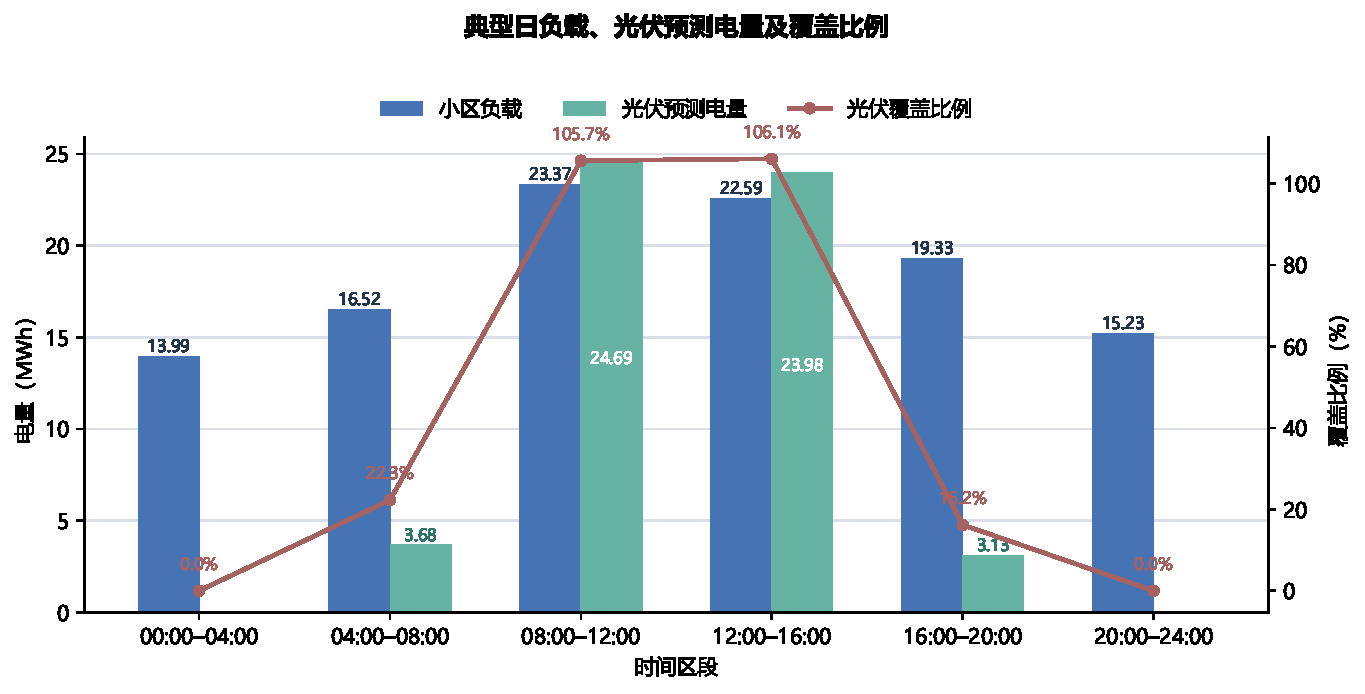
\includegraphics[width=.91\linewidth,height=.63\textheight,keepaspectratio,trim=0 0 0 35bp,clip]{../outputs/figures/paper_v2/q1_load_pv_coverage.pdf}
\renewcommand{\thefigure}{1-2}
\caption{六个4小时区段的负载、光伏预测电量及光伏覆盖比例}\label{fig:q1-2}
\end{figure}

图1-2显示，光伏出力与负载曲线并不同步：部分区段的光伏预测电量能够覆盖较多负载，另一些区段仍存在明显供电缺口。若仅逐时补足净负荷，便无法利用区段前后的能量转移空间，因此需将购电量与储能状态统一纳入跨时段优化。

在明确源荷错位后，还需判断购电计划是否能够响应分时电价。为此，图1-3将净负荷、分时电价与计划购电量置于同一时间轴，并以10分钟阶梯线保留原始调度时间尺度。

\begin{figure}[H]
\centering
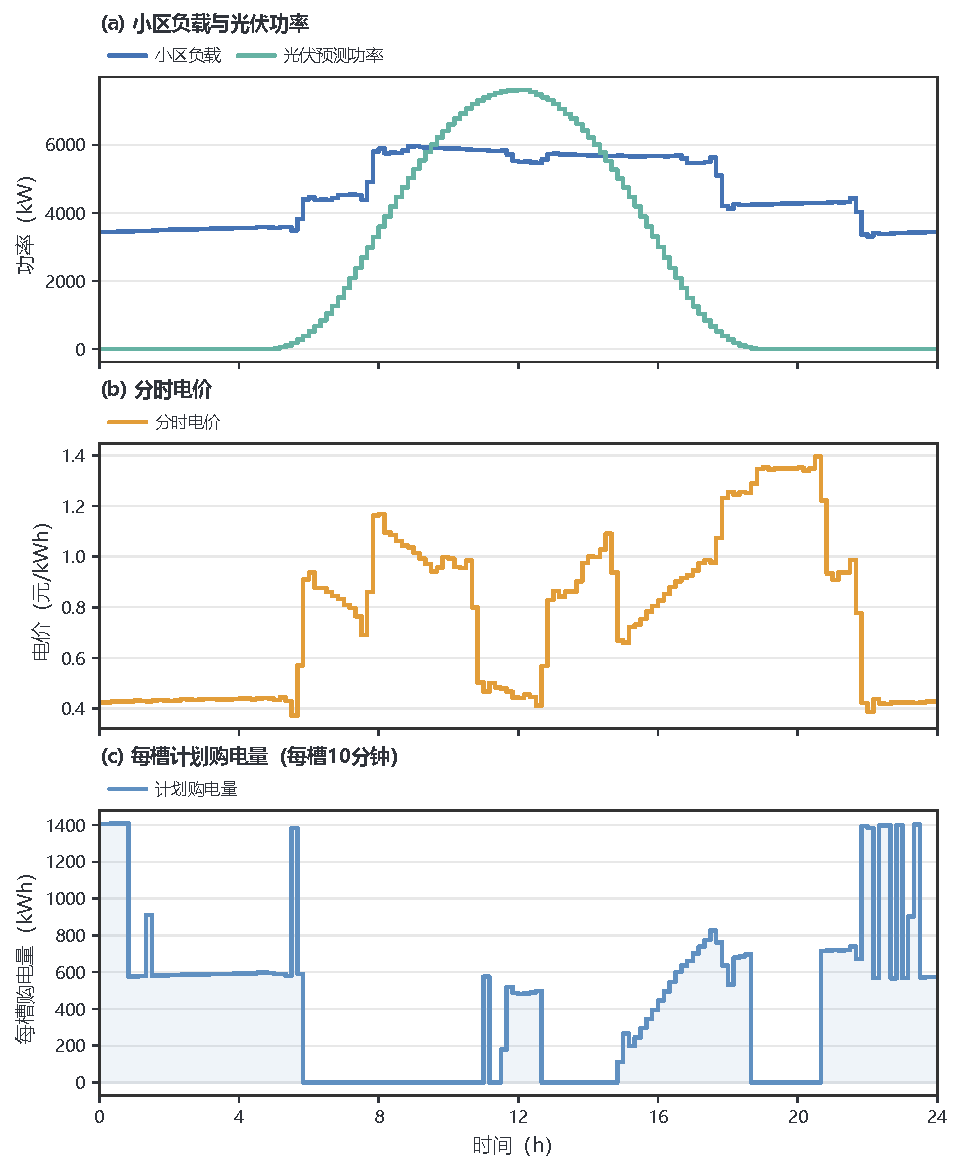
\includegraphics[width=.91\linewidth,height=.63\textheight,keepaspectratio]{../outputs/figures/paper_v2/q1_supply_price_purchase.pdf}
\renewcommand{\thefigure}{1-3}
\caption{净负荷、分时电价与计划购电量（10分钟槽）}\label{fig:q1-3}
\end{figure}

图1-3显示，计划购电量并非简单等于当时净负荷。在部分低价时段，模型适当增加购电并为储能充电；在高价或负荷较高时段，则利用此前储存的电量减少外部购电。费用降低来自电量在时段之间的重新配置，而非削减负载需求。

上述跨时段转移是否可行，最终取决于储能功率及储电量轨迹。图1-4据此展示充放电功率、SOC变化及安全边界。

\begin{figure}[H]
\centering
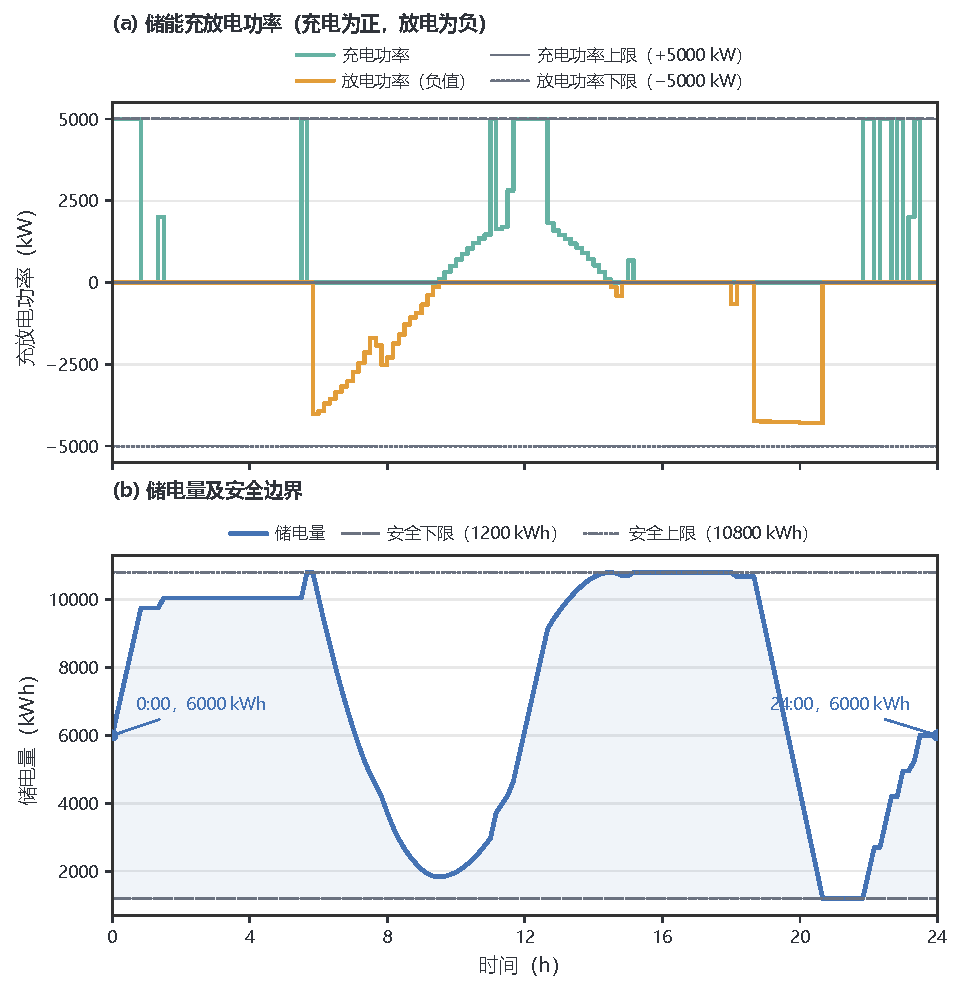
\includegraphics[width=.91\linewidth,height=.63\textheight,keepaspectratio]{../outputs/figures/paper_v2/q1_storage_operation.pdf}
\renewcommand{\thefigure}{1-4}
\caption{充放电功率（正为充电）与连续SOC；虚线为功率和安全边界}\label{fig:q1-4}
\end{figure}

图1-4显示，充、放电动作均未超过功率上限，SOC始终位于安全区间，并在日末恢复至6000 kWh。由此可知，所得费用优势未依赖日末库存透支；问题一的优化方案同时满足物理约束与库存公平性要求。

\subsection{问题二：历史联合残差情景与动态价值调度}\label{ux95eeux9898ux4e8cux5386ux53f2ux8054ux5408ux6b8bux5deeux60c5ux666fux4e0eux52a8ux6001ux4ef7ux503cux8c03ux5ea6}

\subsubsection{历史滚动预测与负载---光伏残差配对}\label{ux5386ux53f2ux6edaux52a8ux9884ux6d4bux4e0eux8d1fux8f7dux5149ux4f0fux6b8bux5deeux914dux5bf9}

下文将问题二的``历史联合残差情景---动态价值调度策略''简称为日前计划---实时执行策略。日前时刻先由已完成历史构造负载与光伏点预测：负载取决策日前35天窗口内同星期几完整日的同槽均值，样本不足时回退到最近至多7个完整日的同槽均值；光伏取最近至多7个完整日的同槽均值。随后仅使用严格早于决策日的完整数据。记相应历史集合为 \(\mathcal H_d^L,\mathcal H_d^G\)，有可用历史样本时，点预测为

\[
\hat L_{d,t}=\frac{1}{|\mathcal H_d^L|}\sum_{j\in\mathcal H_d^L}L_{j,t},\qquad
\hat G_{d,t}=\frac{1}{|\mathcal H_d^G|}\sum_{j\in\mathcal H_d^G}G_{j,t},
\tag{5}
\]

首个可用日的历史集合为空时，按前述规则采用零预测。再按同一历史日配对保留两类残差轨迹；其中 \(\widehat L_{j,t},\widehat G_{j,t}\) 表示历史日 \(j\) 在当时可得信息下形成的点预测，而非目标日 \(d\) 的预测：

\[
r^L_{j,t}=L_{j,t}-\hat L_{j,t},\qquad r^G_{j,t}=G_{j,t}-\hat G_{j,t}.
\tag{5a}
\]

若情景 \(m\) 抽取历史日 \(j_m\)，则目标日的情景供需由点预测叠加该日残差得到：

\[
\widehat L^m_{d,t}=\max\!\left\{0,\widehat L_{d,t}+r^L_{j_m,t}\right\},\qquad
\widehat G^m_{d,t}=\max\!\left\{0,\widehat G_{d,t}+r^G_{j_m,t}\right\}.
\tag{5b}
\]

\subsubsection{完整历史日联合情景构造}\label{ux5b8cux6574ux5386ux53f2ux65e5ux8054ux5408ux60c5ux666fux6784ux9020}

日前购电计划必须在实际负载和光伏尚未完全实现时确定，因此不能直接使用未来真实净负荷。第 \(m\) 个情景的供需量为 \(\hat L_{d,t}+r^L_{j_m,t}\) 与 \(\hat G_{d,t}+r^G_{j_m,t}\)。这种按历史日整体抽取的方式保留负载误差、光伏误差及其日内时序相关性，不把两类残差独立打乱。图2-1展示2025年6月1日的14条历史联合残差轨迹及其生成的净负荷情景带；所有情景均由该决策日之前的信息构造。

\begin{figure}[H]
\centering
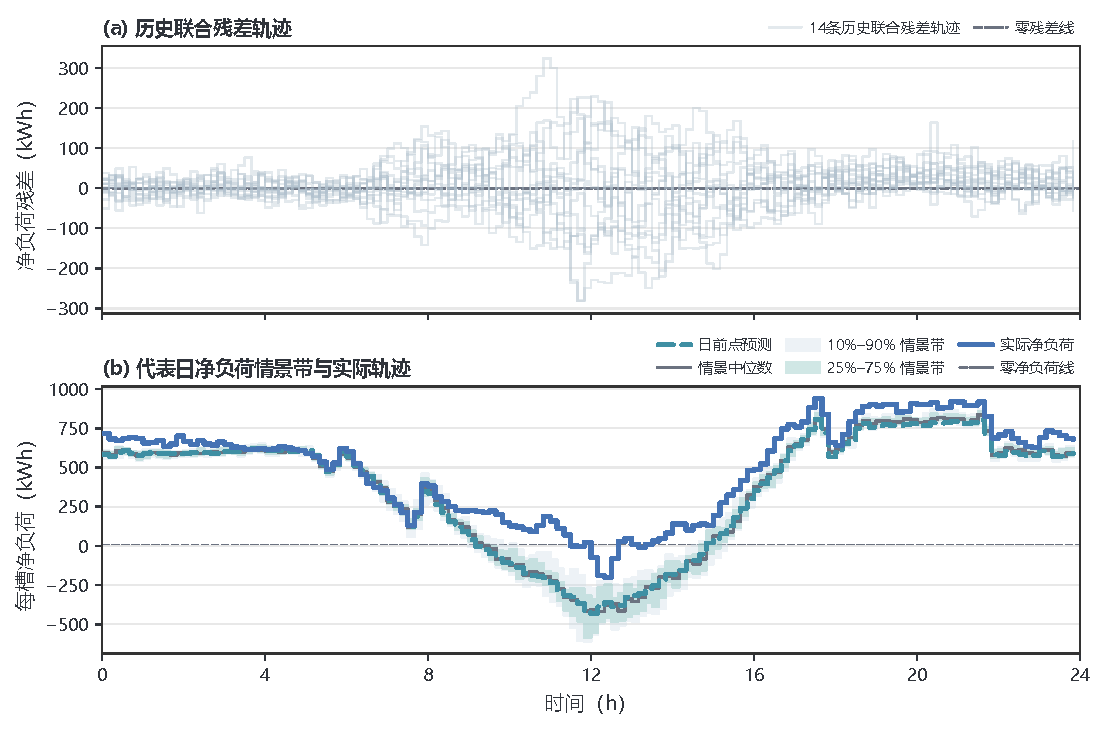
\includegraphics[width=.91\linewidth,height=.63\textheight,keepaspectratio]{../outputs/figures/q2_v2/q2_v2_joint_residual_scenarios.pdf}
\renewcommand{\thefigure}{2-1}
\caption{14条历史净负荷残差轨迹及点预测、情景带与实际净负荷}\label{fig:q2-1}
\end{figure}

各情景总体保持了代表日净负荷的日内变化形态，并在不确定性较强的时段呈现明显离散。实际轨迹在部分时段超出主要情景带，表明有限历史情景不能完全覆盖极端预测偏差；因此，模型保留紧急购电机制，并在实时阶段重新配置储能。

\subsubsection{全情景共同日前购电计划}\label{ux5168ux60c5ux666fux5171ux540cux65e5ux524dux8d2dux7535ux8ba1ux5212}

日前阶段在各情景下优化储能动作，但要求购电计划 \(p_{d,t}\) 对所有情景相同，形成``先决策、后补救''的两阶段情景MILP，而非确定性LP {[}5{]}。目标由计划购电费、情景紧急购电期望成本和终端价值项组成。

两阶段随机混合整数线性规划主要用于确定日前购电计划并评估期望补救费用；情景内补救变量用于刻画不同误差路径下计划的风险后果，并不作为真实日的预见性控制指令。实际运行逐槽观测当前供需和SOC，再由近似价值函数作因果决策。三层变量及跨情景共享关系移列附录A。

令 \(M_d\) 为当日有效情景数，\(E^m_{d,144}\) 为情景 \(m\) 的日末储能电量，日前优化目标可写为

\[
\min J_d=\sum_{t=0}^{143}\pi_t p_{d,t}
+\frac{1}{M_d}\sum_{m=1}^{M_d}\left(\sum_{t=0}^{143}5\pi_t e^m_{d,t}-vE^m_{d,144}\right).
\tag{6a}
\]

各情景分别满足式（1）---（3）、式（2a）---（2b）的储能与供需约束，但共享同一个 \(p_{d,t}\)。只有历史实际量已经完整实现的日期才能进入情景库；样本不足时采用真实有效情景数并重新归一化权重。

其中，第 \(m\) 个情景在每个时段满足

\[
p_{d,t}+\widehat G^m_{d,t}+b^m_{d,t}+e^m_{d,t}
=\widehat L^m_{d,t}+c^m_{d,t}+s^m_{d,t}.
\tag{6b}
\]

各情景均从决策时点真实可得的日初储电量出发，实际执行后的状态再连续传递至下一日：

\[
E^m_{d,0}=E^{\mathrm{actual}}_{d,0},\qquad
E^{\mathrm{actual}}_{d+1,0}=E^{\mathrm{actual}}_{d,144}.
\tag{6c}
\]

式（6b）对全部 \(m=1,\ldots,M_d\) 及 \(t=0,\ldots,143\) 成立。第一阶段变量 \(p_{d,t}\) 在全部情景中保持一致，第二阶段变量随情景变化，由此实现``先计划、后补救''的非预见性结构；式（6c）则区分情景内状态与实际跨日状态。

\subsubsection{近似未来成本与动态价值储能执行}\label{ux8fd1ux4f3cux672aux6765ux6210ux672cux4e0eux52a8ux6001ux4ef7ux503cux50a8ux80fdux6267ux884c}

实时阶段以当前观测到的供需偏差和 SOC 为状态，在历史情景内进行后向递推，得到各路径未来成本函数并取平均，构成近似未来成本。执行器选择使``当前费用+近似未来成本''最小的可行动作；实际SOC不吸附到离散网格。日前SOC计划与实时能量调度相衔接的思路已有工程研究基础{[}6{]}。本文采用离散状态网格近似未来价值，其方法依据可参见近似动态规划专著{[}7{]}及微电网随机动态优化调度研究{[}8{]}，从而让当前动作兼顾后续的紧急购电风险。

设 \(H_t^m(E)\) 为情景路径 \(m\) 上、槽 \(t\) 开始时储能电量为 \(E\) 的未来成本函数。令 \(\mathcal A_t^m(E)\) 为同时满足功率、SOC、供需方向和紧急购电限制的情景可行动作集合，且 \(f(E,a)=E+\eta_c c(a)-b(a)/\eta_d\) 为执行动作 \(a\) 后的SOC。其后向递推及跨情景平均分别为

\[
H_t^m(E)=\min_{a\in\mathcal A_t^m(E)}\left\{5\pi_t e_t^m(a)+H_{t+1}^m\!\left(f(E,a)\right)\right\},
\qquad H_{144}^m(E)=-vE,
\tag{7a}
\]

\[
\overline H_t(E)=\frac{1}{M_d}\sum_{m=1}^{M_d}H_t^m(E).
\tag{7b}
\]

状态为当前SOC，动作 \(a\) 表示充电、放电或保持，即时成本为本槽紧急购电费用，未来成本由决策时点前已经完整实现的历史情景路径近似。实时集合 \(\mathcal A_{d,t}\) 以当前实际净缺口、SOC及功率边界构成；实时动作在该集合内取使下式最小的动作：

\[
a_{d,t}^{\star}\in\arg\min_{a\in\mathcal A_{d,t}}\left\{
5\pi_t e_{d,t}(a)+\overline H_{t+1}\!\left(E_{d,t}+\eta_c c_{d,t}(a)-b_{d,t}(a)/\eta_d\right)
\right\}.
\tag{7c}
\]

式中第一项是当前紧急购电费用，第二项近似保留或释放库存对后续费用的影响。价值函数在离散网格上计算，实际状态只在查询价值时插值，其递推仍保留连续精度。

两阶段模型回答``当天应提前购买多少''，动态价值函数回答``当前槽是否应保留储能电量''。前者控制整体风险，后者处理已经发生的偏差；价值函数基于历史情景路径近似构造，不依赖未来实际轨迹。

\subsubsection{参数确定与独立闭环对照设置}\label{ux53c2ux6570ux786eux5b9aux4e0eux72ecux7acbux95edux73afux5bf9ux7167ux8bbeux7f6e}

参数仅在 1 月开发期选择并冻结：联合残差情景数上限 \(M=14\)、终端库存价值 \(v=0.4\) 元/kWh，SOC 价值函数计算网格为 50 kWh。2---12 月为固定配置的因果影子评价期。为识别执行器贡献，设置贪心储能执行对照：供电富余时尽可能充电、供电不足时在功率和 SOC 边界内尽可能放电，不考虑储能电量的未来机会成本。在相同日前计划和日初 SOC 下的配对消融中，两执行器的差异仅来自实时动作规则；独立跨日闭环比较则允许各自 SOC 与计划连续演化，二者不混合解释。

\subsubsection{全年费用构成与紧急购电时段分配}\label{ux5168ux5e74ux8d39ux7528ux6784ux6210ux4e0eux7d27ux6025ux8d2dux7535ux65f6ux6bb5ux5206ux914d}

为直接回答题目对指定日期的要求，表3汇总相应日期的计划购电量、紧急购电量、实际总费用及日首、日末SOC。由于SOC连续跨日传递，各日结果不仅受当日源荷误差影响，也受到前一日库存状态的影响；六个4小时区段的实际充放电量和逐次紧急购电事件完整列于附录B，正式Excel保留官方模板所需的全部明细。

\begin{longtable}[]{@{}
  >{\centering\arraybackslash}p{(\linewidth - 10\tabcolsep) * \real{0.1304}}
  >{\centering\arraybackslash}p{(\linewidth - 10\tabcolsep) * \real{0.1739}}
  >{\centering\arraybackslash}p{(\linewidth - 10\tabcolsep) * \real{0.1739}}
  >{\centering\arraybackslash}p{(\linewidth - 10\tabcolsep) * \real{0.1739}}
  >{\centering\arraybackslash}p{(\linewidth - 10\tabcolsep) * \real{0.1739}}
  >{\centering\arraybackslash}p{(\linewidth - 10\tabcolsep) * \real{0.1739}}@{}}
\caption{问题二指定日期的购电、费用与SOC汇总}\label{tab:paper-3}\tabularnewline
\toprule\noalign{}
\begin{minipage}[b]{\linewidth}\centering
日期
\end{minipage} & \begin{minipage}[b]{\linewidth}\centering
计划购电量/kWh
\end{minipage} & \begin{minipage}[b]{\linewidth}\centering
紧急购电量/kWh
\end{minipage} & \begin{minipage}[b]{\linewidth}\centering
实际总费用/元
\end{minipage} & \begin{minipage}[b]{\linewidth}\centering
日初SOC/kWh
\end{minipage} & \begin{minipage}[b]{\linewidth}\centering
日末SOC/kWh
\end{minipage} \\
\midrule\noalign{}
\endfirsthead
\toprule\noalign{}
\begin{minipage}[b]{\linewidth}\centering
日期
\end{minipage} & \begin{minipage}[b]{\linewidth}\centering
计划购电量/kWh
\end{minipage} & \begin{minipage}[b]{\linewidth}\centering
紧急购电量/kWh
\end{minipage} & \begin{minipage}[b]{\linewidth}\centering
实际总费用/元
\end{minipage} & \begin{minipage}[b]{\linewidth}\centering
日初SOC/kWh
\end{minipage} & \begin{minipage}[b]{\linewidth}\centering
日末SOC/kWh
\end{minipage} \\
\midrule\noalign{}
\endhead
\bottomrule\noalign{}
\endlastfoot
2025-03-20 & 66,434.776 & 220.145 & 41,727.971 & 1,908.383 & 1,423.256 \\
2025-06-21 & 34,219.048 & 0.000 & 20,206.275 & 3,141.759 & 3,420.893 \\
2025-09-23 & 64,779.270 & 1,867.600 & 51,321.186 & 1,210.074 & 1,375.324 \\
2025-12-21 & 96,029.099 & 0.000 & 61,900.137 & 1,682.761 & 1,759.968 \\
\end{longtable}

表3显示，不同日期的紧急购电水平存在明显差异，表明同一日前策略在不同预测误差下具有不同表现。因此，仅凭少数指定日期不足以评价策略优劣，还需在完整334天因果回放中考察其长期物理状态与经济稳定性。

图2-2首先从绝对运行状态出发，展示主策略全年的SOC分布、月度费用及储能运行特征，用于检验策略是否长期依赖安全边界或异常库存积累；它们均来自同一条334天冻结轨迹。

\begin{figure}[H]
\centering
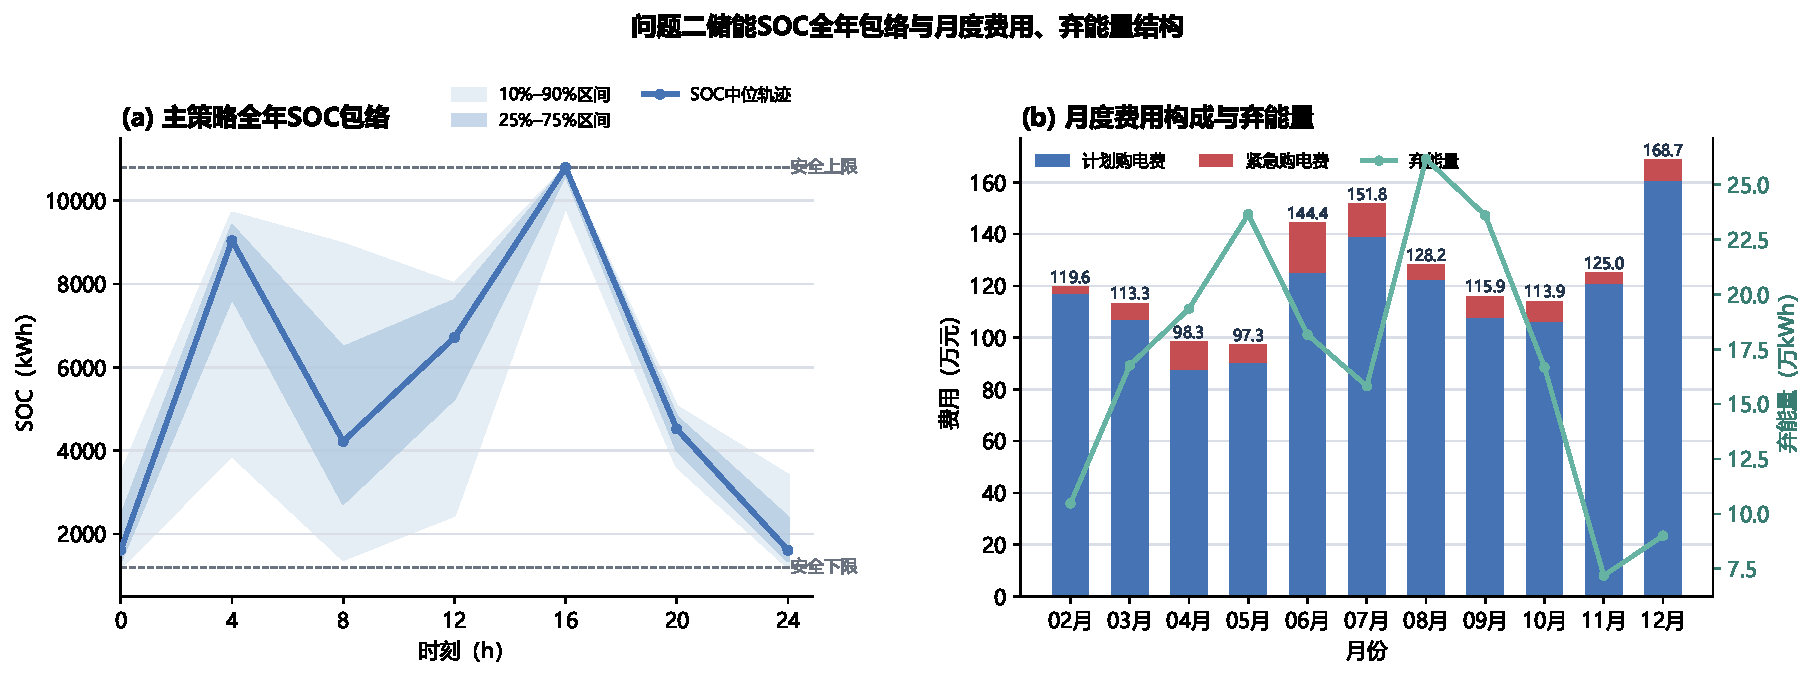
\includegraphics[width=.91\linewidth,height=.63\textheight,keepaspectratio,trim=0 0 0 27bp,clip]{../outputs/figures/q2_v2/q2_v2_soc_envelope_monthly_cost_spill.pdf}
\renewcommand{\thefigure}{2-2}
\caption{全年SOC分位包络、月度费用与弃能量；虚线为SOC安全边界}\label{fig:q2-2}
\end{figure}

全年SOC始终处于安全范围，说明策略具备长期运行可行性；月度费用和弃能量也未显示依赖异常库存积累的情形。但物理可行并不等于经济上优于简单规则，因此图2-3进一步引入贪心执行对照，比较两种执行方式的费用构成、紧急购电价格分布及累计费用差异。

\begin{figure}[H]
\centering
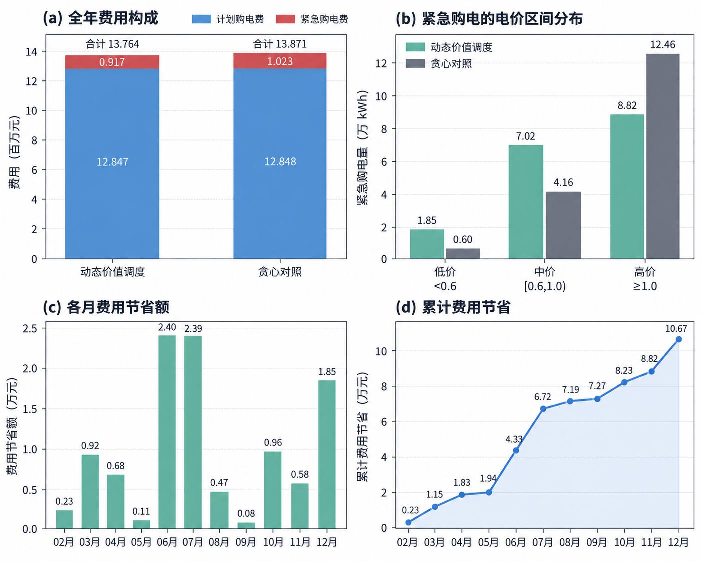
\includegraphics[width=.91\linewidth,height=.54\textheight,keepaspectratio]{../outputs/figures/q2_v2/q2_v2_annual_economic_mechanism.pdf}
\renewcommand{\thefigure}{2-3}
\caption{问题二两种执行策略的费用构成、补购价格分布与累计节省}\label{fig:q2-3}
\end{figure}

这里有一个看似矛盾的现象：日前计划---实时执行策略的紧急购电量由172.161 MWh增至176.902 MWh，实际费用却减少10.666万元。原因不在于减少了所有缺额，而在于改变了缺额出现的时机。按价格区间统计，新增缺额主要落在低、中价时段，而高价时段的紧急购电减少，使加权补购单价由5.942元/kWh降至5.181元/kWh；两种策略的期末SOC相同。可见，储能并非一出现缺额便立即放尽，而是为后续代价更高的时段保留电量。该策略改善的是补购时机，而不只是补购总量。

\subsubsection{最大紧急购电日的储能响应}\label{ux6700ux5927ux7d27ux6025ux8d2dux7535ux65e5ux7684ux50a8ux80fdux54cdux5e94}

为进一步解释上述费用来源，选取全年单日紧急购电量最大的日期作为压力测试日，展示购电、储能功率及SOC的逐时变化，结果见图2-4。

\begin{figure}[H]
\centering
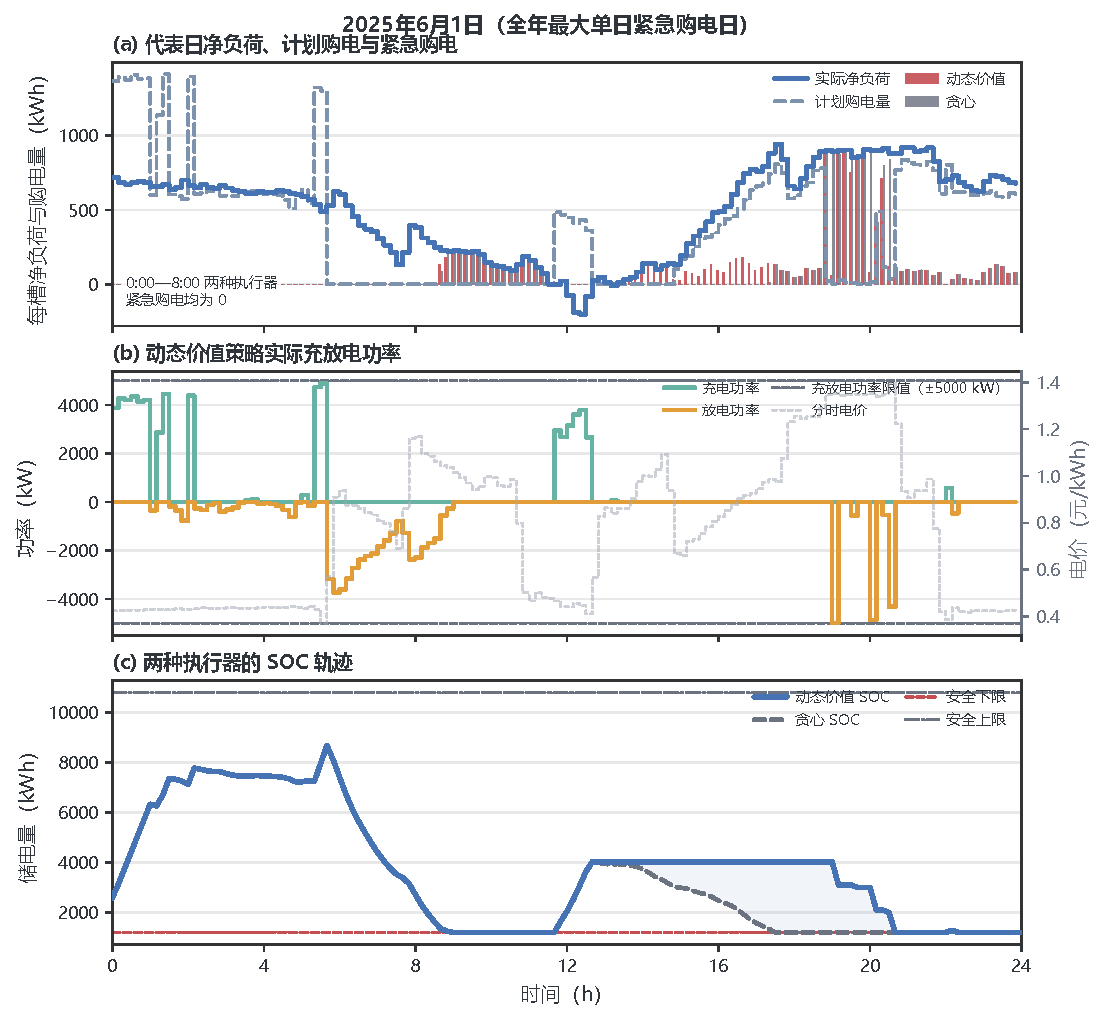
\includegraphics[width=.91\linewidth,height=.56\textheight,keepaspectratio]{../outputs/figures/q2_v2/q2_v2_20250601_dispatch.pdf}
\renewcommand{\thefigure}{2-4}
\caption{2025年6月1日调度：净负荷、购电与补购、储能功率及SOC（负功率为放电）}\label{fig:q2-4}
\end{figure}

代表日轨迹表明，实时执行器需要在当前补购费用与后续库存价值之间进行权衡：部分时段保留储电量，会导致当期出现少量紧急补购，但能够减少后续更高价格时段的补购支出。因此，动态价值策略优化的是紧急购电的时间分布，而非保证每个时段都优先使用储能消除缺口。

\subsection{问题三：多时点预报更新与滚动购电调整}\label{ux95eeux9898ux4e09ux591aux65f6ux70b9ux9884ux62a5ux66f4ux65b0ux4e0eux6edaux52a8ux8d2dux7535ux8c03ux6574}

\subsubsection{发布版本匹配与已执行槽锁定}\label{ux53d1ux5e03ux7248ux672cux5339ux914dux4e0eux5df2ux6267ux884cux69fdux9501ux5b9a}

问题三在问题二基础上增加 0:00、6:00、12:00、18:00 的光伏预报发布与购电计划更新。负载以同星期几历史样本滚动预测；光伏残差相对附件 3 在相同发布时间、相同预测提前量的预报版本计算，并以线性插值映射到 10 分钟槽。每次更新仅使用已发布预报、已完成槽位实测信息和当前 SOC，不能使用尚未完成槽位的实际值。已执行槽随即锁定，后续版本只能修改未执行后缀，且不得追溯改写历史计划。

\subsubsection{未执行计划后缀的滚动优化与结算}\label{ux672aux6267ux884cux8ba1ux5212ux540eux7f00ux7684ux6edaux52a8ux4f18ux5316ux4e0eux7ed3ux7b97}

0:00 求得原计划 \(p_{d,t}\)，在 6:00、12:00、18:00 对未执行后缀重建情景 MILP 和动态价值函数。这种``观测新信息---锁定已执行前缀---优化剩余时域''的处理遵循模型预测控制的滚动时域思想{[}9{]}，并与随机不确定条件下的微网滚动调度研究{[}10{]}一致。令 \(k\in\{0,1,2,3\}\)，按附件官方列序，第 \(k\) 个版本开始生效的列索引为

\[
\rho_k\in\{0,35,71,107\},
\tag{8a}
\]

分别对应0:00、6:00、12:00和18:00。这里的索引指官方00:10、00:20、\ldots\ldots、24:00列从0开始的编号，不改变原始时间列，也不平移正式结果。记 \(z_{d,t}^{(k)}\) 为第 \(k\) 个版本的生效计划，且定义 \(z_{d,t}^{(0)}=p_{d,t}\)。对 \(k=1,2,3\)，已执行前缀满足版本锁定约束

\[
z_{d,t}^{(k)}=z_{d,t}^{(k-1)},\qquad t<\rho_k,
\tag{8b}
\]

而本次滚动求解的初始储电量直接接续真实状态：

\[
E_{d,\rho_k}^{m,(k)}=E_{d,\rho_k}^{\mathrm{actual}},\qquad m=1,\ldots,M_d.
\tag{8c}
\]

后续版本只对 \(t\geq\rho_k\) 的剩余计划求解。其中 \(p_{d,t}\) 始终表示0:00原计划；对 \(k=1,2,3\)，版本计划与原计划之间满足

\[
z_{d,t}^{(k)}=p_{d,t}+\delta_{d,t}^{+,(k)}-\delta_{d,t}^{-,(k)},
\qquad \delta_{d,t}^{+,(k)},\delta_{d,t}^{-,(k)}\ge0,\quad t\geq\rho_k.
\tag{8d}
\]

0:00版本的合同成本为 \(\sum_t\pi_{d,t}p_{d,t}\)。后续版本仅计算尚未执行后缀相对原计划的合同结算项：

\[
 C_{d,\mathrm{contract}}^{(k)}=
 \sum_{t=\rho_k}^{143}\left(\pi_{d,t}p_{d,t}
 +1.5\pi_{d,t}\delta_{d,t}^{+,(k)}
 -0.5\pi_{d,t}\delta_{d,t}^{-,(k)}\right),
\qquad k=1,2,3.
\tag{8e}
\]

已执行时段的账单已经锁定，不再影响本次后缀的最优决策。对 \(k=1,2,3\)，滚动目标为

\[
\min J_d^{(k)}=C_{d,\mathrm{contract}}^{(k)}+
\frac{1}{M_d}\sum_{m=1}^{M_d}\sum_{t=\rho_k}^{143}5\pi_{d,t}e_{d,t}^{m,(k)}
-v\frac{1}{M_d}\sum_{m=1}^{M_d}E_{d,144}^{m,(k)}.
\tag{8f}
\]

相应地，后缀内各情景使用当前版本购电量满足供需平衡：

\[
z_{d,t}^{(k)}+\widehat G_{d,t}^{m,(k)}+b_{d,t}^{m,(k)}+e_{d,t}^{m,(k)}
=\widehat L_{d,t}^{m,(k)}+c_{d,t}^{m,(k)}+s_{d,t}^{m,(k)},\qquad t\geq\rho_k.
\tag{8g}
\]

其余SOC、功率、充放电互斥和紧急购电限制沿用式（1）---（2b）。式（8b）保证后续预报不能追溯改写已执行列，式（8c）则把上一执行区间形成的实际SOC传入下一次优化。执行前最后一次覆盖该列的版本记为最终生效量 \(z_{d,t}\)，并相对0:00原计划定义 \(\delta^+_{d,t}=\max(z_{d,t}-p_{d,t},0)\)、\(\delta^-_{d,t}=\max(p_{d,t}-z_{d,t},0)\)。由于各槽电价为正，若上、下调量同时增加相同电量，式（9）的费用将严格增加，故无需另设调整方向二元变量。

按冻结的透明结算假设，每槽只相对 0:00 原计划结算一次：原计划内电量按正常电价结算，上调部分按1.5倍电价结算，下调部分按原价50\%支付违约成本。

\[
C^{\mathrm{contract}}_{d,t}=\pi_{d,t}p_{d,t}+1.5\pi_{d,t}\delta^+_{d,t}-0.5\pi_{d,t}\delta^-_{d,t},
\tag{9}
\]

\[
C^{\mathrm{emg}}_{d,t}=5\pi_{d,t}e_{d,t}.
\tag{10}
\]

因此，中间计划版本不重复计费；终端库存价值 \(v=0.4\) 元/kWh 仅用于优化目标，不进入实际账单。该调整结算口径是建模解释，不应表述为题目明确给定的唯一合同规则。

式（9）等价于原计划内电量按正常电价结算，上调部分按1.5倍电价结算，下调部分按原电价50\%支付违约成本；它不将中间版本的变动重复计入账单。

若实际市场或题面补充条款明确要求逐版本结算，则应以该规则重新建立费用项；本文结果仅对应上述一次性相对0:00原计划的透明假设。

\subsubsection{共同信息条件下的全年费用比较}\label{ux5171ux540cux4fe1ux606fux6761ux4ef6ux4e0bux7684ux5168ux5e74ux8d39ux7528ux6bd4ux8f83}

在 1 月 22---31 日共同开发期内，以同星期几负载预测、\(M=14\)、\(v=0.4\) 元/kWh、100 kWh 价值网格及四个更新时点确定参数。后文将``多时点预报更新---滚动购电调整与动态价值储能调度策略''简称为滚动调整方案，对照称为禁止调整方案。两者均连续传递实际SOC；对照虽然锁定0:00购电计划，仍按当时可得预报更新储能的未来价值判断。

在评价日内调整机制前，先按照题目规定汇总指定日期结果，见表4。表中同时给出原计划和最终生效购电量、紧急购电量、实际总费用及SOC变化，以反映滚动计划对账单和储能状态的共同影响；指定时刻的原计划与最终生效购电量、六区段实际充放电量和紧急购电事件完整列于附录B。``最终生效''表示该槽执行前最后一个有效计划版本，不累计中间版本调整量。

\begin{longtable}[]{@{}
  >{\centering\arraybackslash}p{(\linewidth - 12\tabcolsep) * \real{0.1111}}
  >{\centering\arraybackslash}p{(\linewidth - 12\tabcolsep) * \real{0.1481}}
  >{\centering\arraybackslash}p{(\linewidth - 12\tabcolsep) * \real{0.1481}}
  >{\centering\arraybackslash}p{(\linewidth - 12\tabcolsep) * \real{0.1481}}
  >{\centering\arraybackslash}p{(\linewidth - 12\tabcolsep) * \real{0.1481}}
  >{\centering\arraybackslash}p{(\linewidth - 12\tabcolsep) * \real{0.1481}}
  >{\centering\arraybackslash}p{(\linewidth - 12\tabcolsep) * \real{0.1481}}@{}}
\caption{问题三指定日期的购电、费用与SOC汇总}\label{tab:paper-4}\tabularnewline
\toprule\noalign{}
\begin{minipage}[b]{\linewidth}\centering
日期
\end{minipage} & \begin{minipage}[b]{\linewidth}\centering
原计划购电量/kWh
\end{minipage} & \begin{minipage}[b]{\linewidth}\centering
最终生效购电量/kWh
\end{minipage} & \begin{minipage}[b]{\linewidth}\centering
紧急购电量/kWh
\end{minipage} & \begin{minipage}[b]{\linewidth}\centering
实际总费用/元
\end{minipage} & \begin{minipage}[b]{\linewidth}\centering
日初SOC/kWh
\end{minipage} & \begin{minipage}[b]{\linewidth}\centering
日末SOC/kWh
\end{minipage} \\
\midrule\noalign{}
\endfirsthead
\toprule\noalign{}
\begin{minipage}[b]{\linewidth}\centering
日期
\end{minipage} & \begin{minipage}[b]{\linewidth}\centering
原计划购电量/kWh
\end{minipage} & \begin{minipage}[b]{\linewidth}\centering
最终生效购电量/kWh
\end{minipage} & \begin{minipage}[b]{\linewidth}\centering
紧急购电量/kWh
\end{minipage} & \begin{minipage}[b]{\linewidth}\centering
实际总费用/元
\end{minipage} & \begin{minipage}[b]{\linewidth}\centering
日初SOC/kWh
\end{minipage} & \begin{minipage}[b]{\linewidth}\centering
日末SOC/kWh
\end{minipage} \\
\midrule\noalign{}
\endhead
\bottomrule\noalign{}
\endlastfoot
2025-03-20 & 69,385.315 & 65,978.619 & 487.478 & 44,213.564 & 1,994.726 & 1,696.363 \\
2025-06-21 & 35,130.641 & 34,194.135 & 0.000 & 19,949.333 & 1,737.956 & 2,644.975 \\
2025-09-23 & 68,873.193 & 66,828.360 & 6.375 & 44,109.288 & 1,480.347 & 1,929.748 \\
2025-12-21 & 96,660.553 & 94,439.918 & 263.191 & 64,278.276 & 1,895.408 & 1,377.915 \\
\end{longtable}

表4中四个指定日期的最终生效总购电量均低于原计划，说明日内更新总体修正了原计划的过量申报；进一步观察附录B中的``问题三指定时刻原计划与最终生效购电量''可见，同一天内仍可能同时存在局部上调和下调，反映模型依据不同时段预测偏差重新配置购电量。为避免用个别日期代替总体结论，下面进一步开展334天独立跨日回放。

图3-1从全年费用构成、紧急购电量及累计节省三个角度，对允许日内调整策略和禁止调整对照进行比较。

\begin{figure}[H]
\centering
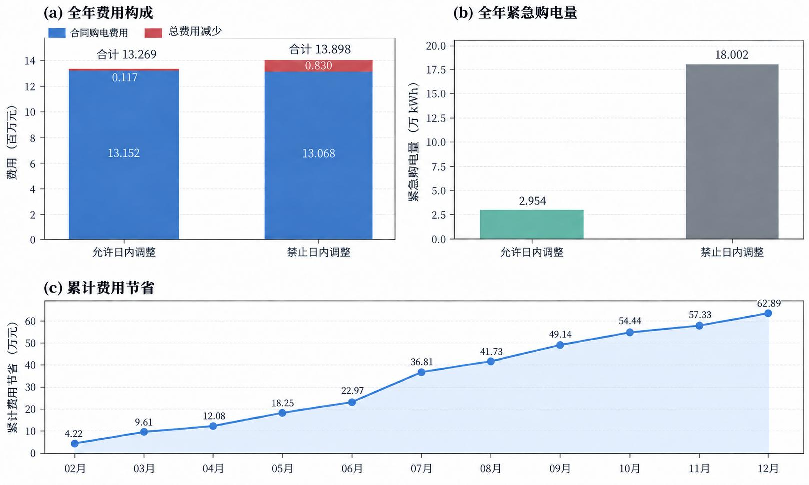
\includegraphics[width=.91\linewidth,height=.63\textheight,keepaspectratio]{../outputs/figures/q3_v2/q3_v2_annual_adjustment_effect.pdf}
\renewcommand{\thefigure}{3-1}
\caption{全年费用、紧急购电量与累计节省；单位分别为百万元、万kWh和万元}\label{fig:q3-1}
\end{figure}

滚动调整方案全年实际费用为1326.878万元，比禁止调整方案少62.894万元，降幅为4.525\%；紧急购电量从180.018 MWh降至29.540 MWh，减少83.590\%。在两方案具有相同预报访问权限的条件下，费用与紧急购电风险均明显下降。因此，从全年经济性和紧急购电风险两个指标来看，利用6:00、12:00和18:00发布的新预报调整尚未执行的购电计划是有必要的。新预报到达后，尚未执行的计划能够及时修正，从而减少后续高成本紧急补缺。两方案的期末SOC并无不利差异，费用改善并非靠消耗更多年末储电量获得。固定计划下的配对试验中，动态价值执行比贪心执行少花12,862.459元；这一数字只刻画给定计划下实时储能判断的作用，不能替代滚动调整带来的全年综合收益。

\subsubsection{代表日计划更新与实际储能运行}\label{ux4ee3ux8868ux65e5ux8ba1ux5212ux66f4ux65b0ux4e0eux5b9eux9645ux50a8ux80fdux8fd0ux884c}

年度指标能够证明滚动调整总体有效，但不能说明一次预报更新如何转化为具体计划。为此，选取2025年3月20日作为代表日，在同一时间轴上展示0:00原计划、三次更新后的计划版本、最终生效计划、储能动作与SOC轨迹，见图3-2。该日为四个指定日期中允许调整策略紧急购电量最大的日期，用于说明机制而不替代全年比较。

\begin{figure}[H]
\centering
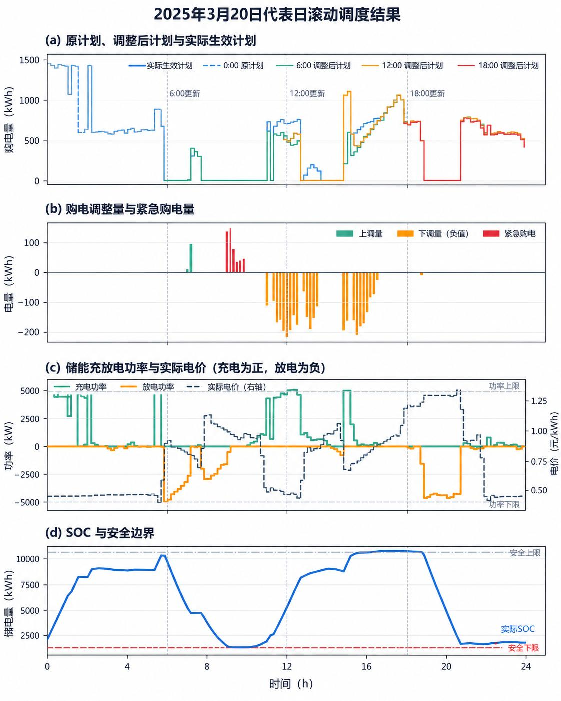
\includegraphics[width=.91\linewidth,height=.55\textheight,keepaspectratio,trim=0 0 0 20bp,clip]{../outputs/figures/q3_v2/q3_v2_20250320_rolling_dispatch.pdf}
\renewcommand{\thefigure}{3-2}
\caption{2025年3月20日滚动调度；竖线为预报更新时间，SOC为连续执行轨迹}\label{fig:q3-2}
\end{figure}

图中竖线对应6:00、12:00和18:00三个预报更新时间。每次更新均只改变尚未执行的计划后缀，更新时刻之前的购电量保持不变，体现了已执行时段锁定原则。计划调整后，储能SOC仍连续递推并保持在安全范围内，说明滚动更新、合同结算与实时储能执行在同一时间链条上保持一致。

\subsection{问题四：波动电价下的因果价格预测与购电调度}\label{ux95eeux9898ux56dbux6ce2ux52a8ux7535ux4ef7ux4e0bux7684ux56e0ux679cux4ef7ux683cux9884ux6d4bux4e0eux8d2dux7535ux8c03ux5ea6}

\subsubsection{价格可用时间与历史同槽均值预测}\label{ux4ef7ux683cux53efux7528ux65f6ux95f4ux4e0eux5386ux53f2ux540cux69fdux5747ux503cux9884ux6d4b}

问题四分别重算问题二型和问题三型策略。本文采用如下价格信息假设：附件4中每个10分钟槽的实际波动电价仅在该槽开始时可知；0:00的计划不能使用目标日未来实际价格，当前槽实际价格只用于实时执行和事后结算。问题4-3在6:00、12:00和18:00更新计划时，沿用当日0:00由完整历史日形成的价格预测曲线，同时更新光伏预报、当前SOC和剩余时域。上述价格可用边界是本文的建模假设，并非题面明文规定。

冻结的价格点预测器为``最近14个完整历史日同槽均值预测''：对待预测槽取此前最多14个完整历史日同一槽的实际价格均值；样本不足时使用当时全部可用的完整日，无历史日时取零预测，并以当日实时价格完成冷启动执行。2月正式评价开始前已经积累完整历史，因此该冷启动分支只影响1月初的状态预热。问题4-2采用 \(M=7\) 个源荷联合残差情景，问题4-3采用 \(M=14\)；两者均采用 \(v=0.6\) 元/kWh和100 kWh价值网格，实际SOC连续递推。

令 \(\mathcal D_d^{14}\) 为日 \(d\) 前最近至多14个已完成日期，则有历史样本时的价格预测为

\[
\widehat\pi_{d,t}=\frac{1}{|\mathcal D_d^{14}|}\sum_{j\in\mathcal D_d^{14}}\pi^{\mathrm{act}}_{j,t}.
\tag{11}
\]

集合 \(\mathcal D_d^{14}\) 不包含目标日；若集合为空，则 \(\widehat\pi_{d,t}=0\)。价格残差由历史实际价减去当时可得的历史预测价得到，不利用全年价格重新拟合历史预测。

具体地，价格预测残差定义为

\[
r_{j,t}^{\pi}=\pi_{j,t}^{\mathrm{act}}-\widehat\pi_{j,t},
\tag{11a}
\]

价格残差只用于评价点预测误差和绘制代表日诊断区间。正式优化中的联合抽样单元由同一完整历史日的负载、光伏残差组成：

\[
\left(r_{j,t}^{L},r_{j,t}^{G}\right)_{t=0}^{143}.
\tag{11b}
\]

两类源荷残差不独立打乱，从而保留负载、光伏误差之间及日内相邻时段的相关性。各供需情景在优化中共用同一条因果价格点预测曲线；因此，现有结果不用于证明价格残差与净负荷残差联合抽样的收益。全部历史样本都来自对应决策日之前已经完整实现的数据。

1月22---31日开发期比较表明，各候选峰值漏判率均为0，但总体误差、高价槽误差和价级识别存在差异。同星期几均值的预测误差最小；最近14个完整日同槽均值同时进入经济回放，并在统一供需预测、场景数、终端价值和网格下取得较低的库存修正费用，故最终采用该方法。由此，预测器选择不是只按MAE排序，也未使用2月以后的正式评价数据。完整预测指标移列附录A。

\subsubsection{日前锁定与日内滚动方案的实际价格结算}\label{ux65e5ux524dux9501ux5b9aux4e0eux65e5ux5185ux6edaux52a8ux65b9ux6848ux7684ux5b9eux9645ux4ef7ux683cux7ed3ux7b97}

问题4-2的正式名称为``波动电价下的源荷联合残差情景---动态价值调度策略''：每天0:00根据因果价格点预测和源荷联合情景制定共同购电计划并全天锁定；实际费用为

\[
C_{4\text{-}2}=\sum_{d,t}\left(\pi^{\mathrm{act}}_{d,t}p_{d,t}+5\pi^{\mathrm{act}}_{d,t}e_{d,t}\right).
\tag{12}
\]

问题 4-3 的正式名称为``波动电价下的多时点滚动购电调整策略''：在 0:00、6:00、12:00、18:00 更新未执行后缀，最终生效量仅相对 0:00 原计划结算一次：

\[
C_{4\text{-}3}=\sum_{d,t}\left(\pi^{\mathrm{act}}_{d,t}p_{d,t}+1.5\pi^{\mathrm{act}}_{d,t}\delta^+_{d,t}-0.5\pi^{\mathrm{act}}_{d,t}\delta^-_{d,t}+5\pi^{\mathrm{act}}_{d,t}e_{d,t}\right).
\tag{13}
\]

预测价格仅作为决策目标中的价格系数，式（12）---（13）统一使用目标槽实际价格结算；库存价值及库存修正费用均不写入正式实际账单。

\subsubsection{高价风险代表日与全年正式综合方案比较}\label{ux9ad8ux4ef7ux98ceux9669ux4ee3ux8868ux65e5ux4e0eux5168ux5e74ux6b63ux5f0fux7efcux5408ux65b9ux6848ux6bd4ux8f83}

波动电价下，策略除面临源荷预测误差外，还需应对未来价格预测误差。为考察价格预测与储能动作的对应关系，本文按全年紧急购电费用最大这一固定规则选取代表日。图4-1依次展示价格点预测及历史残差诊断带、购电计划、储能功率和SOC轨迹。代表日选择和诊断带均只用于事后解释，未参与参数选择；诊断带也未作为正式MILP或价值函数的输入。未来真实电价未进入计划决策，实际价格仅用于当前槽执行和事后结算。

\begin{figure}[H]
\centering
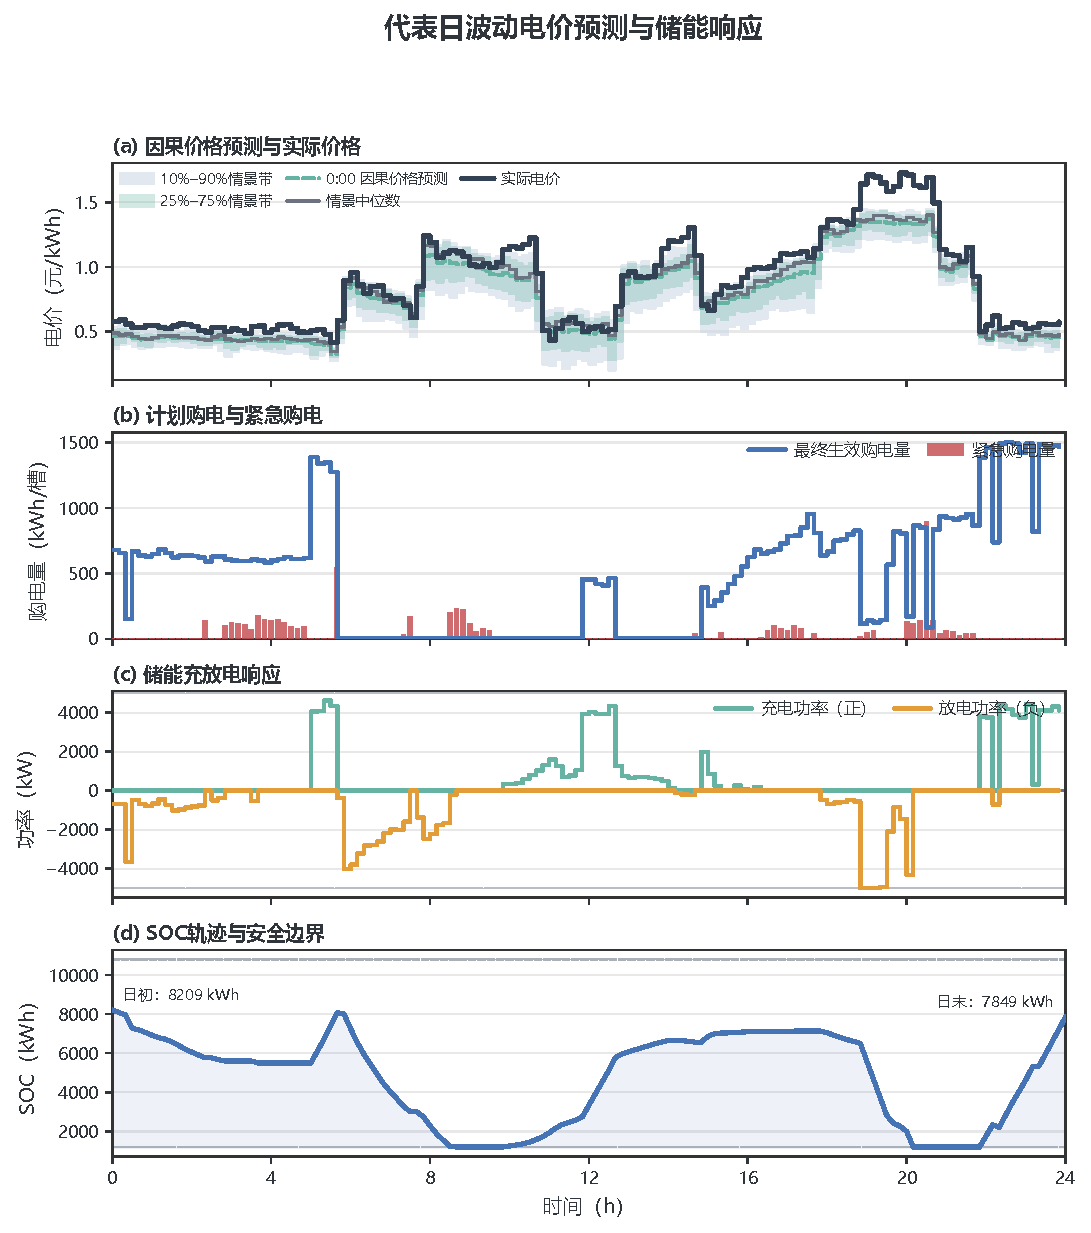
\includegraphics[width=.91\linewidth,height=.63\textheight,keepaspectratio,trim=0 0 0 28bp,clip]{../outputs/figures/q4_v1/q4_v1_representative_price_storage.pdf}
\renewcommand{\thefigure}{4-1}
\caption{2025年7月2日价格预测与储能响应（价格区间为事后诊断带）}\label{fig:q4-1}
\end{figure}

图4-1显示，实际价格在部分时段偏离点预测并超出历史残差诊断区间，表明同槽均值预测不能完全消除价格风险。正式执行依据价格点预测、当前实际供需和近似未来成本安排充放电，而图中的区间仅用于观察误差幅度。全天SOC均满足安全边界，说明该代表日的价格响应未破坏储能物理可行性。

代表日仅用于说明调度机制，问题4-2与问题4-3的总体差异仍须依据完整年度结果判断。精确费用构成、紧急购电量及期末SOC列于附录A``问题四全年费用构成''。为观察费用差异的月度累积过程，并核查比较是否受期末库存影响，图4-2补充展示全年费用构成、紧急购电量、累计费用差和月末SOC。

\begin{figure}[H]
\centering
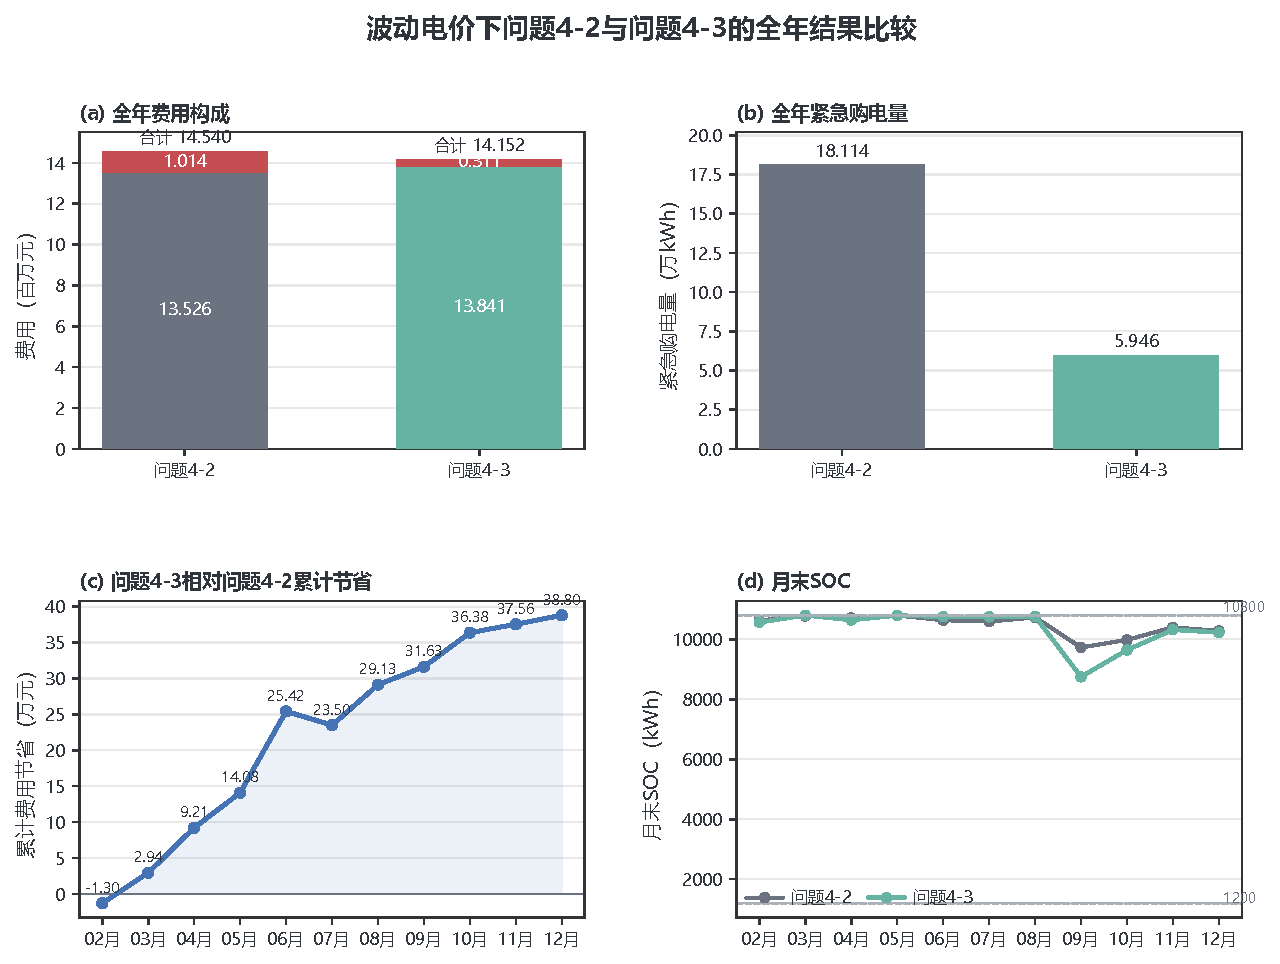
\includegraphics[width=.91\linewidth,height=.63\textheight,keepaspectratio,trim=0 0 0 27bp,clip]{../outputs/figures/q4_v1/q4_v1_annual_comparison.pdf}
\renewcommand{\thefigure}{4-2}
\caption{问题4-2与4-3的全年费用、紧急购电量、累计节省及月末SOC}\label{fig:q4-2}
\end{figure}

在正式综合方案比较中，问题4-3较问题4-2减少费用38.800万元，降幅为2.668\%，紧急购电量减少121.680 MWh，降幅为67.17\%。这一差异反映了滚动更新、价格预测、情景规模和光伏信息来源共同变化后的综合效果。累计差值在年初并非始终为正，随后逐渐形成稳定优势，表明日内更新并不保证每个月均占优，但能够在全年尺度上降低预测偏差带来的高价补购风险。两方案期末SOC接近，采用统一库存修正后费用排序不变。库存公平性统一按 \(C^{\mathrm{inv}}=C^{\mathrm{actual}}+1.0(6000-E_{\mathrm{end}})\) 修正，其中1.0元/kWh参考价在开发期比较前固定，仅用于解释期末SOC差异，不计入实际账单；修正后费用分别为14,535,914.462元和14,147,965.622元，排序不变。

全年共有13次求解在时限内获得可行解，最大相对MIP gap为0.00078259。这些求解均通过供需平衡、SOC递推、功率边界、动作互斥、版本锁定、信息可用时间和费用复算检查，但应如实称为``限时可行解''，不能据此宣称理论全局最优。问题4-2与问题4-3的情景数、光伏信息来源和计划更新机制不同，二者的费用差反映综合方案差异，不能完全归因于单一日内调整机制。为进一步分离日内调整权限本身的作用，第6.5节在完全一致的信息条件和参数下给出独立闭环消融。

\section{模型检验与结果可靠性分析}\label{ux6a21ux578bux68c0ux9a8cux4e0eux7ed3ux679cux53efux9760ux6027ux5206ux6790}

本文将检验分为两类。合规性检查回答``轨迹是否遵循模型、信息边界和结算规则''，其结论仅说明约束得到满足，并不代表策略必然更优；鲁棒性论证则基于开发期已冻结的候选、网格复核和对照轨迹，考察结论是否依赖某一参数或机制。后者仅在已测试范围内解释，不外推为任意扰动下的理论保证。各项方法、数值结果及是否仍需补充试验见附表A-7。

\subsection{能量守恒、SOC递推与费用独立复算}\label{ux80fdux91cfux5b88ux6052socux9012ux63a8ux4e0eux8d39ux7528ux72ecux7acbux590dux7b97}

所有全年轨迹均按334天、48,096个槽逐项核验：日期与官方槽位映射完整，供需平衡和SOC递推残差均处于数值容差内；SOC、功率、充放电互斥及紧急购电同时充电约束均满足；跨日SOC严格衔接；合同费用和紧急购电费用均由逐槽轨迹独立复算。问题三、四另保存预测来源、发布时间和计划版本标记，用于检查信息边界与已执行计划锁定。理论上非负的变量仅在 \([-10^{-6},0)\) kWh范围内规范化为零，低于该阈值的数值视为真实违规。

各方案的最大残差和违规次数集中列于附表A-7，避免正文重复展开验证明细。

\subsection{历史信息可用时间与计划锁定检验}\label{ux5386ux53f2ux4fe1ux606fux53efux7528ux65f6ux95f4ux4e0eux8ba1ux5212ux9501ux5b9aux68c0ux9a8c}

因果性首先由程序的数据筛选逻辑保证：历史残差只从目标日之前的完整日期抽取，光伏预报按发布版本读取，当前槽实际观测仅供实时执行。运行过程中同时记录历史来源、预报发布时间和计划版本生效范围。已有记录未报告未来信息访问或已执行计划改写；但这些运行标记不同于对每个输入时间戳的外部重新计算，因此本文将其作为程序边界检查证据，不扩大解释为形式化证明。

\subsection{开发期参数比较与价值网格敏感性}\label{ux5f00ux53d1ux671fux53c2ux6570ux6bd4ux8f83ux4e0eux4ef7ux503cux7f51ux683cux654fux611fux6027}

参数选择与正式评价按时间分开：1月用于历史积累、连续SOC预热和候选比较，2月1日至12月31日只评价预先固定的策略。情景数、终端库存价值及价值网格的比较沿用已有开发期试验，不根据全年费用追加有利候选。问题二至四的冻结参数表移列附录A；网格仅用于近似价值查询，实际SOC不离散化。已保存的网格复核未改变候选排序：问题二采用50 kWh网格，问题三及问题四采用100 kWh网格。

以终端库存价值 \(v\) 为例，问题二在1月1---31日连续开发回放中，\(v=0,0.4,0.8\) 元/kWh对应实际费用分别为2,381,147.770、2,371,385.460和2,386,137.698元，呈现``过低则低估未来库存、过高则过度保留''的非单调趋势，故在已测试候选中选择0.4元/kWh。该比较共用1月1日初始SOC并连续传递状态，但仍只是开发期证据；不同问题的正式 \(v\) 值见附表A-6，完整敏感性数据见附表A-8。已有网格比较支持以经济表现和计算开销共同选取实现精度，但不能据有限候选试验宣称网格误差已在所有状态上得到理论控制。

\subsection{条件配对消融与独立闭环比较的区别}\label{ux6761ux4ef6ux914dux5bf9ux6d88ux878dux4e0eux72ecux7acbux95edux73afux6bd4ux8f83ux7684ux533aux522b}

条件配对消融固定主策略已经产生的计划轨迹和当日日初SOC，仅更换储能执行规则；独立闭环则让两套方案分别传递自己的实际SOC。问题二条件配对消融中的费用改善为106,662.322元，与独立闭环改善106,661.382元方向一致；问题三条件消融改善为12,862.459元，远小于允许调整方案相对禁止调整对照的总体改善。两种证据分别回答执行规则的条件贡献与整套方案的经济效果，不能相互替代。

\subsection{问题四同信息条件下的日内调整消融}\label{ux95eeux9898ux56dbux540cux4fe1ux606fux6761ux4ef6ux4e0bux7684ux65e5ux5185ux8c03ux6574ux6d88ux878d}

为识别日内购电计划调整的独立贡献，本文开展``问题四同信息条件独立闭环消融''。两分支均从2025年1月1日0:00、SOC=6000 kWh独立启动，共用因果价格预测、负载预测、光伏预报访问权限、14条联合残差情景、终端库存价值、100 kWh价值网格、动态价值执行器及求解设置。锁定方案始终执行0:00原计划；滚动方案在6:00、12:00、18:00仅调整尚未执行的计划后缀。1月按同一规则分别预热并独立传递SOC；正式评价期为2月1日至12月31日，共334天、48,096个10分钟槽。逐槽轨迹显示，两分支2月1日日初SOC均为10,800 kWh；这是各自闭环运行后的观测结果，并非模型强制的共同初值。

经继承一致性审查，正式问题4-3轨迹与公平消融所需rolling分支在初始条件、冻结配置、信息权限、情景构造、求解设置及执行逻辑上完全一致，因此采用正式冻结轨迹作为rolling分支。连续三日的原计划、最终生效计划、充放电、紧急购电、SOC及费用逐槽比较最大误差为\(1.82\times10^{-12}\)，小于既定数值容差；锁定分支另从1月独立运行至年末。表5汇总正式评价期实际账单和期末库存，其中``变化''统一指日内滚动调整减去全天计划锁定。各单元格先用未舍入逐槽值计算，再分别显示到三位小数，故变化列不应由显示值反向相减。库存修正费用仅用于比较年末SOC差异，不替代实际账单。

\begin{longtable}[]{@{}cccc@{}}
\caption{问题四同信息条件独立闭环消融结果}\label{tab:paper-5}\tabularnewline
\toprule\noalign{}
指标 & 全天计划锁定 & 日内滚动调整 & 变化 \\
\midrule\noalign{}
\endfirsthead
\toprule\noalign{}
指标 & 全天计划锁定 & 日内滚动调整 & 变化 \\
\midrule\noalign{}
\endhead
\bottomrule\noalign{}
\endlastfoot
实际总费用/万元 & 1473.773 & 1415.219 & -58.553 \\
合同费用/万元 & 1382.925 & 1384.139 & +1.214 \\
紧急购电费用/万元 & 90.847 & 31.080 & -59.768 \\
紧急购电量/MWh & 173.443 & 59.464 & -113.979 \\
期末SOC/kWh & 10,435.985 & 10,225.682 & -210.302 \\
库存修正费用/万元 & 1473.329 & 1414.797 & -58.532 \\
\end{longtable}

滚动方案的实际费用由1473.773万元降至1415.219万元，按未舍入逐槽账单计算节省585,534.568元，降幅3.973\%；紧急购电量减少113,978.881 kWh，降幅65.715\%。合同费用增加约1.214万元，而紧急购电费用减少约59.768万元，表明新预报的主要经济价值是及时修正未执行计划，降低5倍价格下的紧急补购。334个评价日中，滚动方案胜260天、锁定方案胜69天、持平5天；滚动获胜比例为77.844\%。按统一的1.0元/kWh库存参考价修正后，滚动方案仍节省585,324.265元，费用排序不变。未舍入的完整账单及月度差值见附表A-11和附表A-12。

两分支正式评价期各含48,096槽。锁定方案最大供需平衡残差为\(4.55\times10^{-13}\) kWh、最大SOC递推残差为\(9.09\times10^{-13}\) kWh；SOC与功率越界、同时充放电、紧急购电同时充电均为0，合同与紧急购电费用逐槽复算后的全年总误差为0。锁定方案最大相对MIP gap为0.00036560，有4次限时可行解；复用的滚动方案最大相对gap为0.00078259，有13次限时可行解。历史样本与预报版本按决策时点核对，已执行计划前缀未被改写；上述限时可行解均通过物理及费用核验，但不据此宣称理论全局最优。完整求解状态及日、月结果随支撑材料提供。

\subsection{期末库存公平性与有限时域边界}\label{ux671fux672bux5e93ux5b58ux516cux5e73ux6027ux4e0eux6709ux9650ux65f6ux57dfux8fb9ux754c}

问题二两策略全年末SOC相等；问题三允许调整策略全年末SOC更高。因此，两问中的费用优势均不能解释为期末库存透支。问题四期末SOC虽接近安全上限，但仍处于约束范围内；按事先确定的统一库存参考价修正后，两方案的费用排序不变。终端库存价值会影响有限时域中的保留倾向，高期末库存应作为适用边界说明，不作为真实收入抵扣账单。

\subsection{限时可行解与数值容差}\label{ux9650ux65f6ux53efux884cux89e3ux4e0eux6570ux503cux5bb9ux5dee}

优化求解质量与物理可行性分别报告。日前与滚动MILP均由HiGHS求解，采用单线程和随机种子0；各问题的时限和相对gap请求值按冻结配置执行，逐次求解状态见附表A-7。问题二的334次日前MILP均获得可用解，主策略与贪心对照分别有99次和98次限时可行解，最大报告gap分别为0.00068917和0.00089481；问题三中允许调整策略和禁止调整对照各有86次限时可行解，其余求解均满足请求gap，限时可行解亦通过逐槽物理与费用复算；问题四有13次限时可行解，最大相对MIP gap为0.00078259。最大供需平衡残差、最大SOC递推残差及各类违规次数见附表A-7，四问均未出现超过预设容差的物理违规。这些结果不妨碍逐槽约束与账单独立核验，但均不提供理论精确全局最优保证。理论非负变量只在绝对容差允许的极小负区间内规范化，超过容差的负值视为违规，不能通过无条件截断掩盖。

\subsection{消融对照与已有稳健性证据}\label{ux6d88ux878dux5bf9ux7167ux4e0eux5df2ux6709ux7a33ux5065ux6027ux8bc1ux636e}

本节利用已经冻结的对照轨迹检验关键机制的条件贡献，不将其表述为覆盖任意扰动的全局敏感性结论。首先，问题二在同一购电计划、同一日初SOC和同一信息权限下将动态价值执行替换为因果贪心执行，费用增加106,662.322元；这说明日前计划保持不变时，实时库存价值判断仍具有独立作用。其次，问题三在相同预报权限下将日内更新关闭后，全年费用较允许调整方案增加628,939.753元；而在同计划的条件配对中，仅更换执行器的费用差为12,862.459元，表明两类对照分别识别滚动购电与实时执行的作用，不能混同。

问题四进一步把价格预测器作为反事实对象：两个候选均从2025年1月1日的6000 kWh初始SOC出发并各自连续预热，在相同的10天评价日期、供需预测、情景规模和库存修正口径下，用同星期几历史均值替换最近14个完整日同槽均值，问题4-2型与问题4-3型的库存修正费用分别增加32.972元和1,082.428元，费用排序均未改变。由于不同预测器的预热轨迹会形成不同的1月22日初始SOC，且问题4-2型差异仅约0.0059\%，该结果只说明冻结开发期内的微弱经济排序，不作为显著优势或普遍稳健性的证据。该检验也不等价于``效率降低''或``预测误差任意放大''下的全局敏感性结论；后两类压力测试未在冻结试验中运行，故不作未经计算的数值推断。

为保持正文论证的连续性，本文仅在正文中列出题目要求的指定日期结果和核心机制图。价格预测候选及经济回放见附录A中的``价格预测器的开发期因果误差''和``价格预测器的经济回放''，冻结参数和全年数值验证见``冻结参数与更新范围''及``全年轨迹数值验证''；指定日期六区段充放电结果、指定时刻购电量及紧急购电事件列于附录B。上述材料用于支持参数选择与结果的可复核性，不再参与正式评价期调参。

\section{模型评价与推广}\label{ux6a21ux578bux8bc4ux4ef7ux4e0eux63a8ux5e7f}

\subsection{联合误差刻画与计划---执行分层的优势}\label{ux8054ux5408ux8befux5deeux523bux753bux4e0eux8ba1ux5212ux6267ux884cux5206ux5c42ux7684ux4f18ux52bf}

本文的核心思路包括两点：其一，按完整历史日整体抽取负载与光伏预测误差，避免独立抽样破坏日内时序和源荷关系；其二，以历史情景上的近似价值函数连接日前计划与实时执行。前者使供需情景更接近真实的日内波动，后者避免储能因只顾当前缺额而过早放尽。问题四在此基础上增加因果价格点预测，但没有把价格残差作为正式情景维度。连续跨日SOC进一步保证费用优势不来自每日重置库存。

\subsection{历史情景覆盖与市场结算假设的局限}\label{ux5386ux53f2ux60c5ux666fux8986ux76d6ux4e0eux5e02ux573aux7ed3ux7b97ux5047ux8bbeux7684ux5c40ux9650}

局限包括：历史情景价值函数只是近似未来成本，不能代表完整随机动态规划；光伏预报的整点到 10 分钟映射采用线性插值；有限开发期内选择的窗口、终端价值和网格未必在其他样本上最优；问题三、四的合同调整和电价可用时间均为透明建模解释，可能与实际市场规则不同；限时可行解存在有限 MIP gap。

\subsection{面向实际微网的扩展方向}\label{ux9762ux5411ux5b9eux9645ux5faeux7f51ux7684ux6269ux5c55ux65b9ux5411}

实际应用可在统一能量平衡与计划版本管理框架上增加电池寿命损耗、合同结算条款和预测区间校准。若加入需求响应或设备容量决策，还需重新定义可调负载、投资成本与评价周期，不能把本文运行调度结果直接作为容量配置结论。

\section{结论}\label{ux7ed3ux8bba}

本文围绕光储微网中``提前制定购电计划、实际信息逐步揭示''的核心矛盾，形成了``联合情景刻画不确定性---近似价值函数指导实时执行---版本锁定支持滚动修正''的统一决策链条。问题一在日首、日末储电量均为6000 kWh的约束下实现购电与储能的跨时段协调，单日购电费用为3.513万元。问题二采用完整历史日的联合残差情景制定日前计划，并通过近似未来成本协调实时储能动作；相较贪心执行对照，全年费用降低0.769\%。其收益并非来自机械压缩紧急购电量，而是将部分补购需求由高价时段转移至低、中价时段。问题三利用6:00、12:00和18:00发布的新预报滚动修正尚未执行的购电计划，相较禁止调整对照，全年费用降低4.525\%，紧急购电量减少83.590\%。由此可见，从全年经济性和紧急购电风险两个指标判断，利用三个日内时点的新预报调整购电策略是有必要的。问题四进一步以因果点预测处理未来电价的不确定性；在相同波动电价环境下，问题4-3综合方案较问题4-2综合方案降低费用2.668\%，紧急购电量减少67.17\%，且统一库存修正后比较结论不变。由于两个分支的情景规模、光伏预报信息和计划更新机制不同，该差异反映两套综合方案的表现，不能完全归因于日内调整机制。在控制预测信息、情景参数和储能执行规则后，滚动调整仍获得58.553万元费用节省，验证了日内购电计划修正的独立经济价值。

研究结果表明，储能调度的价值不仅体现在减少紧急购电量，还体现在根据电价和未来供需风险选择储电量的释放时机；联合残差情景能够保留负载与光伏误差的日内相关结构，基于历史情景构造的近似未来成本函数则实现了日前计划与因果实时执行的衔接。需要指出的是，问题二、三采用固定分时电价，问题四采用波动电价，且各问的可用预报、情景规模和更新机制不同，因而不同问题的绝对费用不能直接用于模型优劣排序。后续可结合真实合同结算规则、带有概率校准的价格情景、电池寿命损耗及风险偏好，将现有框架扩展为风险约束或多目标调度模型。

\section*{AI工具使用声明}

本参赛队在竞赛过程中使用了AI工具，主要用于代码调试、图表制作、文字润色和一致性检查{[}11{]}，详细使用情况见支撑材料。模型设定、程序运行、参数选择、数值复算、结果解释和最终论文内容均由参赛队逐项审核并承担责任。

\section*{参考文献}

{[}1{]} Elkazaz M, Sumner M, Thomas D. Energy management system for hybrid PV-wind-battery microgrid using convex programming, model predictive and rolling horizon predictive control with experimental validation{[}J{]}. \emph{International Journal of Electrical Power \& Energy Systems}, 2020, 115: 105483. DOI: 10.1016/j.ijepes.2019.105483.

{[}2{]} Conejo A J, Carrión M, Morales J M. \emph{Decision Making Under Uncertainty in Electricity Markets}. New York: Springer, 2010.

{[}3{]} Silvente J, Kopanos G M, Pistikopoulos E N, Espuña A. A rolling horizon optimization framework for the simultaneous energy supply and demand planning in microgrids{[}J{]}. \emph{Applied Energy}, 2015, 155: 485-501. DOI: 10.1016/j.apenergy.2015.05.090.

{[}4{]} 殷辉，陆信辉，周开乐. 分布式与集中式储能并存的微电网负荷优化调度{[}J{]}. 中国管理科学，2023，31(2)：118-128. DOI: 10.16381/j.cnki.issn1003-207x.2020.0762.

{[}5{]} Birge J R, Louveaux F. \emph{Introduction to Stochastic Programming}, 2nd ed.~New York: Springer, 2011.

{[}6{]} 孟晓丽，牛焕娜，贾东梨，等. 基于储能SOC日前计划的微电网实时能量优化调度方法{[}J{]}. 农业工程学报，2016，32(8)：155-161. DOI: 10.11975/j.issn.1002-6819.2016.08.022.

{[}7{]} Powell W B. \emph{Approximate Dynamic Programming: Solving the Curses of Dimensionality}, 2nd ed.~Hoboken: John Wiley \& Sons, 2011.

{[}8{]} 王雅平，林舜江，杨智斌，等. 微电网多目标随机动态优化调度算法{[}J{]}. 电工技术学报，2018，33(10)：2196-2207. DOI: 10.19595/j.cnki.1000-6753.tces.170496.

{[}9{]} Rawlings J B, Mayne D Q, Diehl M M. \emph{Model Predictive Control: Theory, Computation, and Design}, 2nd ed.~Madison: Nob Hill Publishing, 2017.

{[}10{]} Silvente J, Kopanos G M, Dua V, Papageorgiou L G. A rolling horizon approach for optimal management of microgrids under stochastic uncertainty{[}J{]}. \emph{Chemical Engineering Research and Design}, 2018, 131: 293-317. DOI: 10.1016/j.cherd.2017.09.013.

{[}11{]} OpenAI Codex，GPT-5，OpenAI，2026-09-06---2026-09-13。

\clearpage\appendix\section*{附录}

\subsection*{附录A 参数候选与补充验证材料}

正式结果以题目模板输出。问题二、三、四的参数均在各自 1 月开发期选定并冻结，后续全年仅进行因果评价；正式账单均不扣除终端库存价值。参数开发遵循``预测筛选---经济回放---网格复核---冻结评价''的顺序，所有候选共用初始SOC、评价日期、信息权限和求解设置。

滚动求解与实时执行的核心步骤如下：（1）在决策时点截取已可用历史与已发布预报；（2）按完整历史日构造联合残差情景；（3）求解跨情景共享的购电计划或未执行后缀；（4）锁定已执行槽并以当前真实SOC初始化；（5）重建近似未来价值函数并逐槽执行；（6）按实际价格和最终生效计划独立结算；（7）保存SOC、历史库、计划版本和累计账单检查点。任何未来信息访问、真实负变量违规或无可行解均触发停止，而不以回退规则掩盖。

\par\pagebreak[2]\subsubsection*{A.1 问题二的规划与执行层次}

\begingroup\renewcommand{\tablename}{附表}\renewcommand{\thetable}{A-1}

\begin{longtable}[]{@{}cccc@{}}
\caption{问题二的规划与执行层次}\label{tab:appendix-A-1}\tabularnewline
\toprule\noalign{}
决策层 & 决策时刻 & 主要变量 & 跨情景共享 \\
\midrule\noalign{}
\endfirsthead
\toprule\noalign{}
决策层 & 决策时刻 & 主要变量 & 跨情景共享 \\
\midrule\noalign{}
\endhead
\bottomrule\noalign{}
\endlastfoot
第一阶段 & 当日0:00 & 计划购电量 \(p_{d,t}\) & 是 \\
第二阶段 & 各联合情景 & 充电、放电、紧急购电、弃能及SOC & 否 \\
实时执行 & 每个10分钟槽 & 实际充放电与紧急购电 & 不属于日前轨迹 \\
\end{longtable}

\endgroup

\par\pagebreak[2]\subsubsection*{A.2 问题二与问题三全年策略比较}

\begingroup\renewcommand{\tablename}{附表}\renewcommand{\thetable}{A-2}

\begin{longtable}[]{@{}
  >{\centering\arraybackslash}p{(\linewidth - 8\tabcolsep) * \real{0.1667}}
  >{\centering\arraybackslash}p{(\linewidth - 8\tabcolsep) * \real{0.1667}}
  >{\centering\arraybackslash}p{(\linewidth - 8\tabcolsep) * \real{0.2222}}
  >{\centering\arraybackslash}p{(\linewidth - 8\tabcolsep) * \real{0.2222}}
  >{\centering\arraybackslash}p{(\linewidth - 8\tabcolsep) * \real{0.2222}}@{}}
\caption{问题二与问题三全年策略比较}\label{tab:appendix-A-2}\tabularnewline
\toprule\noalign{}
\begin{minipage}[b]{\linewidth}\centering
问题
\end{minipage} & \begin{minipage}[b]{\linewidth}\centering
策略
\end{minipage} & \begin{minipage}[b]{\linewidth}\centering
实际总费用/元
\end{minipage} & \begin{minipage}[b]{\linewidth}\centering
紧急购电量/kWh
\end{minipage} & \begin{minipage}[b]{\linewidth}\centering
期末SOC/kWh
\end{minipage} \\
\midrule\noalign{}
\endfirsthead
\toprule\noalign{}
\begin{minipage}[b]{\linewidth}\centering
问题
\end{minipage} & \begin{minipage}[b]{\linewidth}\centering
策略
\end{minipage} & \begin{minipage}[b]{\linewidth}\centering
实际总费用/元
\end{minipage} & \begin{minipage}[b]{\linewidth}\centering
紧急购电量/kWh
\end{minipage} & \begin{minipage}[b]{\linewidth}\centering
期末SOC/kWh
\end{minipage} \\
\midrule\noalign{}
\endhead
\bottomrule\noalign{}
\endlastfoot
问题二 & 历史联合残差情景---动态价值调度 & 13,763,928.208 & 176,902.132 & 1,404.800 \\
& 贪心执行对照 & 13,870,589.590 & 172,161.349 & 1,404.800 \\
问题三 & 允许日内调整 & 13,268,776.239 & 29,540.082 & 1,462.576 \\
& 禁止日内调整对照 & 13,897,715.992 & 180,018.160 & 1,399.588 \\
\end{longtable}

\endgroup

\par\pagebreak[2]\subsubsection*{A.3 价格预测器的开发期因果误差}

\begingroup\renewcommand{\tablename}{附表}\renewcommand{\thetable}{A-3}

\begin{longtable}[]{@{}
  >{\centering\arraybackslash}p{(\linewidth - 12\tabcolsep) * \real{0.1071}}
  >{\centering\arraybackslash}p{(\linewidth - 12\tabcolsep) * \real{0.1429}}
  >{\centering\arraybackslash}p{(\linewidth - 12\tabcolsep) * \real{0.1429}}
  >{\centering\arraybackslash}p{(\linewidth - 12\tabcolsep) * \real{0.1429}}
  >{\centering\arraybackslash}p{(\linewidth - 12\tabcolsep) * \real{0.1429}}
  >{\centering\arraybackslash}p{(\linewidth - 12\tabcolsep) * \real{0.1429}}
  >{\centering\arraybackslash}p{(\linewidth - 12\tabcolsep) * \real{0.1786}}@{}}
\caption{价格预测器的开发期因果误差}\label{tab:appendix-A-3}\tabularnewline
\toprule\noalign{}
\begin{minipage}[b]{\linewidth}\centering
价格预测方法
\end{minipage} & \begin{minipage}[b]{\linewidth}\centering
MAE
\end{minipage} & \begin{minipage}[b]{\linewidth}\centering
RMSE
\end{minipage} & \begin{minipage}[b]{\linewidth}\centering
高价槽MAE
\end{minipage} & \begin{minipage}[b]{\linewidth}\centering
峰值漏判率/\%
\end{minipage} & \begin{minipage}[b]{\linewidth}\centering
价级准确率/\%
\end{minipage} & \begin{minipage}[b]{\linewidth}\centering
采用
\end{minipage} \\
\midrule\noalign{}
\endfirsthead
\toprule\noalign{}
\begin{minipage}[b]{\linewidth}\centering
价格预测方法
\end{minipage} & \begin{minipage}[b]{\linewidth}\centering
MAE
\end{minipage} & \begin{minipage}[b]{\linewidth}\centering
RMSE
\end{minipage} & \begin{minipage}[b]{\linewidth}\centering
高价槽MAE
\end{minipage} & \begin{minipage}[b]{\linewidth}\centering
峰值漏判率/\%
\end{minipage} & \begin{minipage}[b]{\linewidth}\centering
价级准确率/\%
\end{minipage} & \begin{minipage}[b]{\linewidth}\centering
采用
\end{minipage} \\
\midrule\noalign{}
\endhead
\bottomrule\noalign{}
\endlastfoot
上一可用日同槽价格 & 0.08973 & 0.13349 & 0.07918 & 0.00 & 85.28 & \\
最近7个完整日同槽均值 & 0.08357 & 0.10709 & 0.07771 & 0.00 & 83.96 & \\
最近14个完整日同槽均值 & 0.08228 & 0.10744 & 0.07412 & 0.00 & 85.28 & √ \\
指数加权移动预测 & 0.08755 & 0.11449 & 0.07805 & 0.00 & 83.13 & \\
同星期几历史均值 & 0.03478 & 0.04482 & 0.03446 & 0.00 & 95.21 & \\
\end{longtable}

\endgroup

前三项误差单位均为元/kWh。最终方法由预测筛选和经济回放共同确定。

\par\pagebreak[2]\subsubsection*{A.4 价格预测器的经济回放}

在统一的同星期几供需预测、\(M=14\)、\(v=0.2\) 元/kWh与100 kWh价值网格下，仅将预测指标较优且风险特征不同的两个候选进入10天开发期经济回放。两种预测器共享2025年1月1日6000 kWh的预热起点和1月22---31日评价日期，但各自连续预热后形成的评价期初SOC并不相同；库存修正口径在比较前固定。

\begingroup\renewcommand{\tablename}{附表}\renewcommand{\thetable}{A-4}

\begin{longtable}[]{@{}
  >{\centering\arraybackslash}p{(\linewidth - 8\tabcolsep) * \real{0.1667}}
  >{\centering\arraybackslash}p{(\linewidth - 8\tabcolsep) * \real{0.1667}}
  >{\centering\arraybackslash}p{(\linewidth - 8\tabcolsep) * \real{0.2222}}
  >{\centering\arraybackslash}p{(\linewidth - 8\tabcolsep) * \real{0.2222}}
  >{\centering\arraybackslash}p{(\linewidth - 8\tabcolsep) * \real{0.2222}}@{}}
\caption{价格预测器的经济回放}\label{tab:appendix-A-4}\tabularnewline
\toprule\noalign{}
\begin{minipage}[b]{\linewidth}\centering
分支
\end{minipage} & \begin{minipage}[b]{\linewidth}\centering
价格预测方法
\end{minipage} & \begin{minipage}[b]{\linewidth}\centering
10天实际费用/元
\end{minipage} & \begin{minipage}[b]{\linewidth}\centering
库存修正费用/元
\end{minipage} & \begin{minipage}[b]{\linewidth}\centering
期末SOC/kWh
\end{minipage} \\
\midrule\noalign{}
\endfirsthead
\toprule\noalign{}
\begin{minipage}[b]{\linewidth}\centering
分支
\end{minipage} & \begin{minipage}[b]{\linewidth}\centering
价格预测方法
\end{minipage} & \begin{minipage}[b]{\linewidth}\centering
10天实际费用/元
\end{minipage} & \begin{minipage}[b]{\linewidth}\centering
库存修正费用/元
\end{minipage} & \begin{minipage}[b]{\linewidth}\centering
期末SOC/kWh
\end{minipage} \\
\midrule\noalign{}
\endhead
\bottomrule\noalign{}
\endlastfoot
问题4-2型 & 同星期几历史均值 & 552,710.227 & 556,874.705 & 1,835.522 \\
& 最近14个完整日同槽均值 & 552,651.576 & 556,841.734 & 1,809.842 \\
问题4-3型 & 同星期几历史均值 & 545,290.952 & 549,697.051 & 1,593.901 \\
& 最近14个完整日同槽均值 & 544,223.348 & 548,614.623 & 1,608.726 \\
\end{longtable}

\endgroup

两分支中，最近14个完整日同槽均值的库存修正费用均较低，因而按冻结开发流程选为正式评价的价格预测器。问题4-2型的修正费用仅低32.972元，约0.0059\%，属于微小差异；该选择不否定同星期几历史均值在点预测指标和期末SOC上的优势，也不把开发期排序外推为普遍结论。

\par\pagebreak[2]\subsubsection*{A.5 问题四全年费用构成}

\begingroup\renewcommand{\tablename}{附表}\renewcommand{\thetable}{A-5}

\begin{longtable}[]{@{}ccc@{}}
\caption{问题四全年费用构成}\label{tab:appendix-A-5}\tabularnewline
\toprule\noalign{}
指标 & 问题4-2 & 问题4-3 \\
\midrule\noalign{}
\endfirsthead
\toprule\noalign{}
指标 & 问题4-2 & 问题4-3 \\
\midrule\noalign{}
\endhead
\bottomrule\noalign{}
\endlastfoot
合同（计划）结算费用/元 & 13,525,826.803 & 13,841,394.701 \\
紧急购电费用/元 & 1,014,367.047 & 310,796.603 \\
实际总费用/元 & 14,540,193.850 & 14,152,191.304 \\
紧急购电量/kWh & 181,144.015 & 59,464.119 \\
期末SOC/kWh & 10,279.388 & 10,225.682 \\
\end{longtable}

\endgroup

\par\pagebreak[2]\subsubsection*{A.6 冻结参数与更新范围}

\begingroup\renewcommand{\tablename}{附表}\renewcommand{\thetable}{A-6}

\begin{longtable}[]{@{}ccccc@{}}
\caption{冻结参数与更新范围}\label{tab:appendix-A-6}\tabularnewline
\toprule\noalign{}
模型 & 情景数上限 & 终端价值/（元/kWh） & 价值网格/kWh & 计划更新 \\
\midrule\noalign{}
\endfirsthead
\toprule\noalign{}
模型 & 情景数上限 & 终端价值/（元/kWh） & 价值网格/kWh & 计划更新 \\
\midrule\noalign{}
\endhead
\bottomrule\noalign{}
\endlastfoot
问题二 & 14 & 0.4 & 50 & 仅0:00 \\
问题三 & 14 & 0.4 & 100 & 0:00、6:00、12:00、18:00 \\
问题4-2 & 7 & 0.6 & 100 & 仅0:00 \\
问题4-3 & 14 & 0.6 & 100 & 0:00、6:00、12:00、18:00 \\
\end{longtable}

\endgroup

\par\pagebreak[2]\subsubsection*{A.7 全年轨迹数值验证}

\begingroup\renewcommand{\tablename}{附表}\renewcommand{\thetable}{A-7}

\begin{longtable}[]{@{}
  >{\centering\arraybackslash}p{(\linewidth - 12\tabcolsep) * \real{0.1111}}
  >{\centering\arraybackslash}p{(\linewidth - 12\tabcolsep) * \real{0.1481}}
  >{\centering\arraybackslash}p{(\linewidth - 12\tabcolsep) * \real{0.1481}}
  >{\centering\arraybackslash}p{(\linewidth - 12\tabcolsep) * \real{0.1481}}
  >{\centering\arraybackslash}p{(\linewidth - 12\tabcolsep) * \real{0.1481}}
  >{\centering\arraybackslash}p{(\linewidth - 12\tabcolsep) * \real{0.1481}}
  >{\centering\arraybackslash}p{(\linewidth - 12\tabcolsep) * \real{0.1481}}@{}}
\caption{全年轨迹数值验证}\label{tab:appendix-A-7}\tabularnewline
\toprule\noalign{}
\begin{minipage}[b]{\linewidth}\centering
方案
\end{minipage} & \begin{minipage}[b]{\linewidth}\centering
最大供需残差/kWh
\end{minipage} & \begin{minipage}[b]{\linewidth}\centering
最大SOC递推残差/kWh
\end{minipage} & \begin{minipage}[b]{\linewidth}\centering
SOC违规
\end{minipage} & \begin{minipage}[b]{\linewidth}\centering
功率违规
\end{minipage} & \begin{minipage}[b]{\linewidth}\centering
同时充放电
\end{minipage} & \begin{minipage}[b]{\linewidth}\centering
边界日志异常
\end{minipage} \\
\midrule\noalign{}
\endfirsthead
\toprule\noalign{}
\begin{minipage}[b]{\linewidth}\centering
方案
\end{minipage} & \begin{minipage}[b]{\linewidth}\centering
最大供需残差/kWh
\end{minipage} & \begin{minipage}[b]{\linewidth}\centering
最大SOC递推残差/kWh
\end{minipage} & \begin{minipage}[b]{\linewidth}\centering
SOC违规
\end{minipage} & \begin{minipage}[b]{\linewidth}\centering
功率违规
\end{minipage} & \begin{minipage}[b]{\linewidth}\centering
同时充放电
\end{minipage} & \begin{minipage}[b]{\linewidth}\centering
边界日志异常
\end{minipage} \\
\midrule\noalign{}
\endhead
\bottomrule\noalign{}
\endlastfoot
问题二 & \(6.821\times10^{-13}\) & \(4.537\times10^{-12}\) & 0 & 0 & 0 & 0 \\
问题三允许调整 & \(1.999\times10^{-10}\) & \(1.462\times10^{-10}\) & 0 & 0 & 0 & 0 \\
问题4-2 & \(6.821\times10^{-13}\) & \(4.547\times10^{-12}\) & 0 & 0 & 0 & 0 \\
问题4-3 & \(6.821\times10^{-13}\) & \(4.547\times10^{-12}\) & 0 & 0 & 0 & 0 \\
\end{longtable}

\endgroup

\par\pagebreak[2]\subsubsection*{A.8 终端库存价值敏感性}

问题二以2025年1月1日相同初始SOC=6000 kWh出发，采用100 kWh价值网格连续回放至1月31日；终端库存价值只进入优化，不计入下表实际费用。不同 \(v\) 会改变月末SOC，因此表中未修正账单同时反映费用和库存保留差异。

\begingroup\renewcommand{\tablename}{附表}\renewcommand{\thetable}{A-8}

\begin{longtable}[]{@{}
  >{\centering\arraybackslash}p{(\linewidth - 8\tabcolsep) * \real{0.2000}}
  >{\raggedright\arraybackslash}p{(\linewidth - 8\tabcolsep) * \real{0.2000}}
  >{\raggedright\arraybackslash}p{(\linewidth - 8\tabcolsep) * \real{0.2000}}
  >{\raggedright\arraybackslash}p{(\linewidth - 8\tabcolsep) * \real{0.2000}}
  >{\centering\arraybackslash}p{(\linewidth - 8\tabcolsep) * \real{0.2000}}@{}}
\caption{终端库存价值敏感性}\label{tab:appendix-A-8}\tabularnewline
\toprule\noalign{}
\begin{minipage}[b]{\linewidth}\centering
\(v\)/（元/kWh）
\end{minipage} & \begin{minipage}[b]{\linewidth}\raggedright
实际费用/元
\end{minipage} & \begin{minipage}[b]{\linewidth}\raggedright
相对 \(v=0.4\) 的变化/元
\end{minipage} & \begin{minipage}[b]{\linewidth}\raggedright
1月末SOC/kWh
\end{minipage} & \begin{minipage}[b]{\linewidth}\centering
价值网格/kWh
\end{minipage} \\
\midrule\noalign{}
\endfirsthead
\toprule\noalign{}
\begin{minipage}[b]{\linewidth}\centering
\(v\)/（元/kWh）
\end{minipage} & \begin{minipage}[b]{\linewidth}\raggedright
实际费用/元
\end{minipage} & \begin{minipage}[b]{\linewidth}\raggedright
相对 \(v=0.4\) 的变化/元
\end{minipage} & \begin{minipage}[b]{\linewidth}\raggedright
1月末SOC/kWh
\end{minipage} & \begin{minipage}[b]{\linewidth}\centering
价值网格/kWh
\end{minipage} \\
\midrule\noalign{}
\endhead
\bottomrule\noalign{}
\endlastfoot
0 & 2,381,147.770 & +9,762.310 & 1,620.082 & 100 \\
0.4 & 2,371,385.460 & 0 & 1,781.855 & 100 \\
0.8 & 2,386,137.698 & +14,752.238 & 10,800.000 & 100 \\
\end{longtable}

\endgroup

已测试候选显示未修正费用随 \(v\) 呈非单调变化，同时较大的 \(v\) 明显提高了月末库存。该结论只支持在该开发设置与测试点 \(\{0,0.4,0.8\}\) 中进行比较，不能单独由未修正账单断言库存价值过高或过低；若需讨论0.2或0.6等中间取值，须在相同开发期、网格和库存修正口径下另行试验，不得借正式评价期结果选参。

\par\pagebreak[2]\subsubsection*{A.9 问题4-3全年调整结算构成}

\begingroup\renewcommand{\tablename}{附表}\renewcommand{\thetable}{A-9}

\begin{longtable}[]{@{}cc@{}}
\caption{问题4-3全年调整结算构成}\label{tab:appendix-A-9}\tabularnewline
\toprule\noalign{}
指标 & 数值 \\
\midrule\noalign{}
\endfirsthead
\toprule\noalign{}
指标 & 数值 \\
\midrule\noalign{}
\endhead
\bottomrule\noalign{}
\endlastfoot
0:00原计划购电量/kWh & 21,217,032.615 \\
最终生效购电量/kWh & 20,687,390.914 \\
上调量/kWh & 266,843.009 \\
下调量/kWh & 796,484.711 \\
0:00原计划对应费用/元 & 13,829,545.820 \\
上调附加费用/元 & 284,507.144 \\
下调退款金额/元 & 272,658.262 \\
最终合同结算费用/元 & 13,841,394.701 \\
紧急购电费用/元 & 310,796.603 \\
实际总费用/元 & 14,152,191.304 \\
非零调整槽数 & 7,256 \\
零调整槽数 & 40,840 \\
\end{longtable}

\endgroup

上表按每槽最终生效量相对0:00原计划结算一次；上调附加费用和下调退款均未累计中间计划版本，终端库存价值也未进入实际账单。

\par\pagebreak[2]\subsubsection*{A.10 问题4-3限时可行解明细}

\begingroup\renewcommand{\tablename}{附表}\renewcommand{\thetable}{A-10}

\begin{longtable}[]{@{}
  >{\centering\arraybackslash}p{(\linewidth - 10\tabcolsep) * \real{0.1304}}
  >{\centering\arraybackslash}p{(\linewidth - 10\tabcolsep) * \real{0.1739}}
  >{\centering\arraybackslash}p{(\linewidth - 10\tabcolsep) * \real{0.1739}}
  >{\centering\arraybackslash}p{(\linewidth - 10\tabcolsep) * \real{0.1739}}
  >{\centering\arraybackslash}p{(\linewidth - 10\tabcolsep) * \real{0.1739}}
  >{\centering\arraybackslash}p{(\linewidth - 10\tabcolsep) * \real{0.1739}}@{}}
\caption{问题4-3限时可行解明细}\label{tab:appendix-A-10}\tabularnewline
\toprule\noalign{}
\begin{minipage}[b]{\linewidth}\centering
日期
\end{minipage} & \begin{minipage}[b]{\linewidth}\centering
发布时间
\end{minipage} & \begin{minipage}[b]{\linewidth}\centering
incumbent/元
\end{minipage} & \begin{minipage}[b]{\linewidth}\centering
best bound/元
\end{minipage} & \begin{minipage}[b]{\linewidth}\centering
相对gap
\end{minipage} & \begin{minipage}[b]{\linewidth}\centering
求解时间/s
\end{minipage} \\
\midrule\noalign{}
\endfirsthead
\toprule\noalign{}
\begin{minipage}[b]{\linewidth}\centering
日期
\end{minipage} & \begin{minipage}[b]{\linewidth}\centering
发布时间
\end{minipage} & \begin{minipage}[b]{\linewidth}\centering
incumbent/元
\end{minipage} & \begin{minipage}[b]{\linewidth}\centering
best bound/元
\end{minipage} & \begin{minipage}[b]{\linewidth}\centering
相对gap
\end{minipage} & \begin{minipage}[b]{\linewidth}\centering
求解时间/s
\end{minipage} \\
\midrule\noalign{}
\endhead
\bottomrule\noalign{}
\endlastfoot
2025-03-01 & 0:00 & 12,070.420 & 12,067.527 & 0.00023965 & 45.544 \\
2025-04-15 & 0:00 & 25,407.488 & 25,404.830 & 0.00010463 & 45.798 \\
2025-04-27 & 12:00 & 16,341.134 & 16,328.345 & 0.00078259 & 45.730 \\
2025-05-05 & 0:00 & 29,891.056 & 29,883.970 & 0.00023704 & 45.961 \\
2025-06-11 & 0:00 & 46,947.622 & 46,934.994 & 0.00026899 & 46.220 \\
2025-08-05 & 0:00 & 49,081.738 & 49,076.257 & 0.00011166 & 46.272 \\
2025-08-21 & 0:00 & 45,213.456 & 45,205.439 & 0.00017729 & 46.737 \\
2025-09-10 & 0:00 & 42,606.230 & 42,597.288 & 0.00020988 & 46.216 \\
2025-09-15 & 0:00 & 29,648.260 & 29,639.771 & 0.00028630 & 46.208 \\
2025-09-18 & 0:00 & 31,799.674 & 31,781.624 & 0.00056760 & 46.744 \\
2025-09-25 & 0:00 & 35,902.672 & 35,897.575 & 0.00014196 & 46.203 \\
2025-10-07 & 0:00 & 33,138.153 & 33,134.211 & 0.00011894 & 46.724 \\
2025-12-24 & 0:00 & 63,929.343 & 63,920.876 & 0.00013244 & 46.250 \\
\end{longtable}

\endgroup

13次求解均在时限内获得满足物理约束的可行解，其中最大相对gap为0.00078259；本文不将其称为已证明的理论最优解。

\par\pagebreak[2]\subsubsection*{A.11 问题四同信息条件独立闭环消融完整结果}

两方案均在2025年1月1日0:00以SOC=6000 kWh启动，各自完成1月预热；2月1日日初SOC均为10,800.000 kWh。下表仅汇总2月1日至12月31日的334天账单，费用以元列出；正式问题4-3轨迹经继承一致性审查后只读复用为日内滚动调整分支。变化定义为滚动减锁定，库存修正值按\(C^{\mathrm{actual}}+1.0(6000-E_{\mathrm{end}})\)计算。

\begingroup\renewcommand{\tablename}{附表}\renewcommand{\thetable}{A-11}

\begin{longtable}[]{@{}cccc@{}}
\caption{问题四同信息条件独立闭环消融完整结果}\label{tab:appendix-A-11}\tabularnewline
\toprule\noalign{}
指标 & 全天计划锁定 & 日内滚动调整 & 变化 \\
\midrule\noalign{}
\endfirsthead
\toprule\noalign{}
指标 & 全天计划锁定 & 日内滚动调整 & 变化 \\
\midrule\noalign{}
\endhead
\bottomrule\noalign{}
\endlastfoot
实际总费用/元 & 14,737,725.872 & 14,152,191.304 & -585,534.568 \\
合同费用/元 & 13,829,253.712 & 13,841,394.701 & +12,140.990 \\
紧急购电费用/元 & 908,472.161 & 310,796.603 & -597,675.558 \\
紧急购电量/kWh & 173,443.000 & 59,464.119 & -113,978.881 \\
期末SOC/kWh & 10,435.985 & 10,225.682 & -210.302 \\
库存修正费用/元 & 14,733,289.887 & 14,147,965.622 & -585,324.265 \\
费用较锁定方案下降/\% & --- & 3.973 & --- \\
紧急购电量较锁定方案下降/\% & --- & 65.715 & --- \\
费用胜出日数/天 & 69 & 260 & --- \\
费用持平日数/天 & 5 & 5 & --- \\
限时可行解/次 & 4 & 13 & --- \\
最大相对MIP gap & 0.00036560 & 0.00078259 & --- \\
\end{longtable}

\endgroup

表内各分项分别由未舍入逐槽值汇总后显示到三位小数；若以显示值反向相减出现0.001元差异，以高精度逐槽汇总为准，不调整正式账单。

\par\pagebreak[2]\subsubsection*{A.12 问题四同信息条件独立闭环消融月度费用差}

月度差和累计差均为``全天计划锁定费用－日内滚动调整费用''；正值表示滚动方案节省。各月费用来自正式评价期的逐日账单，不含1月预热费用。

\begingroup\renewcommand{\tablename}{附表}\renewcommand{\thetable}{A-12}

\begin{longtable}[]{@{}ccc@{}}
\caption{问题四同信息条件独立闭环消融月度费用差}\label{tab:appendix-A-12}\tabularnewline
\toprule\noalign{}
月份 & 月度费用差/万元 & 累计费用差/万元 \\
\midrule\noalign{}
\endfirsthead
\toprule\noalign{}
月份 & 月度费用差/万元 & 累计费用差/万元 \\
\midrule\noalign{}
\endhead
\bottomrule\noalign{}
\endlastfoot
2月 & 5.768 & 5.768 \\
3月 & 5.840 & 11.608 \\
4月 & 3.171 & 14.778 \\
5月 & 4.612 & 19.391 \\
6月 & 2.450 & 21.840 \\
7月 & 13.385 & 35.225 \\
8月 & 4.839 & 40.064 \\
9月 & 4.895 & 44.959 \\
10月 & 4.733 & 49.692 \\
11月 & 3.064 & 52.756 \\
12月 & 5.798 & 58.553 \\
\end{longtable}

\endgroup

\subsection*{附录B 指定日期与全年轨迹材料}

正文表3和表4给出指定日期摘要；以下附表列出题目要求的六个4小时区段实际充放电量。充电量与放电量均为非负kWh幅值，SOC按实际连续轨迹取日初与日末状态。

\clearpage\subsubsection*{B.1 问题二指定日期六区段充放电量及SOC}

\begingroup\renewcommand{\tablename}{附表}\renewcommand{\thetable}{B-1}

\begin{longtable}[]{@{}cccccc@{}}
\caption{问题二指定日期六区段充放电量及SOC}\label{tab:appendix-B-1}\tabularnewline
\toprule\noalign{}
日期 & 时间段 & 充电量/kWh & 放电量/kWh & 日初SOC/kWh & 日末SOC/kWh \\
\midrule\noalign{}
\endfirsthead
\toprule\noalign{}
日期 & 时间段 & 充电量/kWh & 放电量/kWh & 日初SOC/kWh & 日末SOC/kWh \\
\midrule\noalign{}
\endhead
\bottomrule\noalign{}
\endlastfoot
2025-03-20 & 0:00---4:00 & 8,204.256 & 279.948 & 1,908.383 & 1,423.256 \\
& 4:00---8:00 & 1,759.177 & 5,041.105 & & \\
& 8:00---12:00 & 5,368.419 & 2,777.377 & & \\
& 12:00---16:00 & 4,863.455 & 374.397 & & \\
& 16:00---20:00 & 96.795 & 5,781.283 & & \\
& 20:00---24:00 & 455.410 & 2,987.989 & & \\
2025-06-21 & 0:00---4:00 & 1,129.252 & 365.616 & 3,141.759 & 3,420.893 \\
& 4:00---8:00 & 1,295.056 & 2,400.854 & & \\
& 8:00---12:00 & 6,611.356 & 0.000 & & \\
& 12:00---16:00 & 2,888.889 & 0.000 & & \\
& 16:00---20:00 & 53.055 & 4,949.496 & & \\
& 20:00---24:00 & 1,009.039 & 2,551.996 & & \\
2025-09-23 & 0:00---4:00 & 8,786.725 & 258.250 & 1,210.074 & 1,375.324 \\
& 4:00---8:00 & 1,619.807 & 5,851.127 & & \\
& 8:00---12:00 & 4,583.227 & 1,896.616 & & \\
& 12:00---16:00 & 5,569.566 & 646.611 & & \\
& 16:00---20:00 & 4.741 & 5,894.436 & & \\
& 20:00---24:00 & 463.663 & 2,336.695 & & \\
2025-12-21 & 0:00---4:00 & 8,648.515 & 222.049 & 1,682.761 & 1,759.968 \\
& 4:00---8:00 & 2,674.476 & 1,514.425 & & \\
& 8:00---12:00 & 5,539.033 & 6,943.709 & & \\
& 12:00---16:00 & 6,725.393 & 2,220.109 & & \\
& 16:00---20:00 & 17.253 & 5,585.580 & & \\
& 20:00---24:00 & 447.826 & 2,927.161 & & \\
\end{longtable}

\endgroup

\par\pagebreak[2]\subsubsection*{B.2 问题三指定日期六区段充放电量及SOC}

\begingroup\renewcommand{\tablename}{附表}\renewcommand{\thetable}{B-2}

\begin{longtable}[]{@{}cccccc@{}}
\caption{问题三指定日期六区段充放电量及SOC}\label{tab:appendix-B-2}\tabularnewline
\toprule\noalign{}
日期 & 时间段 & 充电量/kWh & 放电量/kWh & 日初SOC/kWh & 日末SOC/kWh \\
\midrule\noalign{}
\endfirsthead
\multicolumn{6}{c}{\small 续附表B-2 问题三指定日期六区段充放电量及SOC}\\
\toprule\noalign{}
日期 & 时间段 & 充电量/kWh & 放电量/kWh & 日初SOC/kWh & 日末SOC/kWh \\
\midrule\noalign{}
\endhead
\bottomrule\noalign{}
\endlastfoot
2025-03-20 & 0:00---4:00 & 7,832.865 & 141.135 & 1,994.726 & 1,696.363 \\
& 4:00---8:00 & 1,768.054 & 6,060.963 & & \\
& 8:00---12:00 & 4,463.046 & 2,289.899 & & \\
& 12:00---16:00 & 6,404.927 & 254.723 & & \\
& 16:00---20:00 & 114.670 & 5,413.157 & & \\
& 20:00---24:00 & 433.524 & 3,132.488 & & \\
2025-06-21 & 0:00---4:00 & 1,072.299 & 44.795 & 1,737.956 & 2,644.975 \\
& 4:00---8:00 & 1,128.547 & 1,721.408 & & \\
& 8:00---12:00 & 3,604.145 & 0.000 & & \\
& 12:00---16:00 & 6,444.444 & 0.000 & & \\
& 16:00---20:00 & 16.598 & 5,563.264 & & \\
& 20:00---24:00 & 989.192 & 2,590.948 & & \\
2025-09-23 & 0:00---4:00 & 8,383.883 & 155.428 & 1,480.347 & 1,929.748 \\
& 4:00---8:00 & 2,058.053 & 5,014.253 & & \\
& 8:00---12:00 & 4,248.012 & 1,896.616 & & \\
& 12:00---16:00 & 4,915.240 & 426.218 & & \\
& 16:00---20:00 & 19.460 & 5,971.175 & & \\
& 20:00---24:00 & 762.390 & 2,645.350 & & \\
2025-12-21 & 0:00---4:00 & 8,332.366 & 205.848 & 1,895.408 & 1,377.915 \\
& 4:00---8:00 & 2,594.578 & 1,718.794 & & \\
& 8:00---12:00 & 5,298.848 & 7,268.264 & & \\
& 12:00---16:00 & 7,839.392 & 2,285.760 & & \\
& 16:00---20:00 & 8.355 & 6,033.491 & & \\
& 20:00---24:00 & 304.666 & 2,699.932 & & \\
\end{longtable}

\endgroup

\par\pagebreak[2]\subsubsection*{B.3 问题二指定时刻计划购电量}

\begingroup\renewcommand{\tablename}{附表}\renewcommand{\thetable}{B-3}

\begin{longtable}[]{@{}ccccccc@{}}
\caption{问题二指定时刻计划购电量}\label{tab:appendix-B-3}\tabularnewline
\toprule\noalign{}
日期 & 10:00 & 12:00 & 14:00 & 16:00 & 18:00 & 20:00 \\
\midrule\noalign{}
\endfirsthead
\toprule\noalign{}
日期 & 10:00 & 12:00 & 14:00 & 16:00 & 18:00 & 20:00 \\
\midrule\noalign{}
\endhead
\bottomrule\noalign{}
\endlastfoot
2025-03-20 & 0.000 & 725.215 & 0.000 & 450.981 & 697.983 & 0.000 \\
2025-06-21 & 0.000 & 0.000 & 0.000 & 111.599 & 356.846 & 0.000 \\
2025-09-23 & 0.000 & 508.351 & 0.000 & 459.218 & 731.594 & 12.994 \\
2025-12-21 & 0.000 & 924.766 & 0.000 & 804.412 & 711.214 & 0.000 \\
\end{longtable}

\endgroup

\par\pagebreak[2]\subsubsection*{B.4 问题三指定时刻原计划与最终生效购电量}

\begingroup\renewcommand{\tablename}{附表}\renewcommand{\thetable}{B-4}

\begin{longtable}[]{@{}
  >{\centering\arraybackslash}p{(\linewidth - 14\tabcolsep) * \real{0.1000}}
  >{\centering\arraybackslash}p{(\linewidth - 14\tabcolsep) * \real{0.1000}}
  >{\centering\arraybackslash}p{(\linewidth - 14\tabcolsep) * \real{0.1333}}
  >{\centering\arraybackslash}p{(\linewidth - 14\tabcolsep) * \real{0.1333}}
  >{\centering\arraybackslash}p{(\linewidth - 14\tabcolsep) * \real{0.1333}}
  >{\centering\arraybackslash}p{(\linewidth - 14\tabcolsep) * \real{0.1333}}
  >{\centering\arraybackslash}p{(\linewidth - 14\tabcolsep) * \real{0.1333}}
  >{\centering\arraybackslash}p{(\linewidth - 14\tabcolsep) * \real{0.1333}}@{}}
\caption{问题三指定时刻原计划与最终生效购电量}\label{tab:appendix-B-4}\tabularnewline
\toprule\noalign{}
\begin{minipage}[b]{\linewidth}\centering
日期
\end{minipage} & \begin{minipage}[b]{\linewidth}\centering
版本
\end{minipage} & \begin{minipage}[b]{\linewidth}\centering
10:00
\end{minipage} & \begin{minipage}[b]{\linewidth}\centering
12:00
\end{minipage} & \begin{minipage}[b]{\linewidth}\centering
14:00
\end{minipage} & \begin{minipage}[b]{\linewidth}\centering
16:00
\end{minipage} & \begin{minipage}[b]{\linewidth}\centering
18:00
\end{minipage} & \begin{minipage}[b]{\linewidth}\centering
20:00
\end{minipage} \\
\midrule\noalign{}
\endfirsthead
\multicolumn{8}{c}{\small 续附表B-4 问题三指定时刻原计划与最终生效购电量}\\
\toprule\noalign{}
\begin{minipage}[b]{\linewidth}\centering
日期
\end{minipage} & \begin{minipage}[b]{\linewidth}\centering
版本
\end{minipage} & \begin{minipage}[b]{\linewidth}\centering
10:00
\end{minipage} & \begin{minipage}[b]{\linewidth}\centering
12:00
\end{minipage} & \begin{minipage}[b]{\linewidth}\centering
14:00
\end{minipage} & \begin{minipage}[b]{\linewidth}\centering
16:00
\end{minipage} & \begin{minipage}[b]{\linewidth}\centering
18:00
\end{minipage} & \begin{minipage}[b]{\linewidth}\centering
20:00
\end{minipage} \\
\midrule\noalign{}
\endhead
\bottomrule\noalign{}
\endlastfoot
2025-03-20 & 0:00原计划 & 0.000 & 692.520 & 0.000 & 693.681 & 695.290 & 0.000 \\
& 最终生效计划 & 0.000 & 498.058 & 0.000 & 524.767 & 695.290 & 0.000 \\
2025-06-21 & 0:00原计划 & 0.000 & 0.000 & 0.000 & 89.347 & 393.930 & 0.000 \\
& 最终生效计划 & 0.000 & 0.000 & 0.000 & 57.088 & 375.151 & 0.000 \\
2025-09-23 & 0:00原计划 & 0.000 & 359.795 & 0.000 & 521.323 & 728.115 & 12.994 \\
& 最终生效计划 & 0.000 & 0.000 & 0.000 & 506.038 & 768.934 & 28.107 \\
2025-12-21 & 0:00原计划 & 0.000 & 1,090.816 & 0.000 & 846.986 & 709.805 & 0.000 \\
& 最终生效计划 & 0.000 & 881.730 & 0.000 & 846.986 & 686.760 & 0.000 \\
\end{longtable}

\endgroup

\par\pagebreak[2]\subsubsection*{B.5 指定日期紧急购电事件}

\begingroup\renewcommand{\tablename}{附表}\renewcommand{\thetable}{B-5}

\begin{longtable}[]{@{}cccc@{}}
\caption{指定日期紧急购电事件}\label{tab:appendix-B-5}\tabularnewline
\toprule\noalign{}
问题 & 日期 & 紧急购电时间段 & 紧急购电量/kWh \\
\midrule\noalign{}
\endfirsthead
\toprule\noalign{}
问题 & 日期 & 紧急购电时间段 & 紧急购电量/kWh \\
\midrule\noalign{}
\endhead
\bottomrule\noalign{}
\endlastfoot
问题二 & 2025-03-20 & 17:10---17:30 & 43.936 \\
问题二 & 2025-03-20 & 20:20---20:50 & 110.180 \\
问题二 & 2025-03-20 & 21:40---22:00 & 66.030 \\
问题二 & 2025-06-21 & 无 & 0.000 \\
问题二 & 2025-09-23 & 16:40---17:00 & 87.127 \\
问题二 & 2025-09-23 & 17:10---18:00 & 193.519 \\
问题二 & 2025-09-23 & 18:20---19:00 & 267.203 \\
问题二 & 2025-09-23 & 20:20---22:10 & 1,319.752 \\
问题二 & 2025-12-21 & 无 & 0.000 \\
问题三 & 2025-03-20 & 9:10---10:10 & 487.478 \\
问题三 & 2025-06-21 & 无 & 0.000 \\
问题三 & 2025-09-23 & 20:30---20:40 & 6.375 \\
问题三 & 2025-12-21 & 20:20---21:00 & 238.475 \\
问题三 & 2025-12-21 & 21:40---22:00 & 24.716 \\
\end{longtable}

\endgroup

\clearpage\subsubsection*{B.6 问题二与问题三指定日期费用分解}

\begingroup\renewcommand{\tablename}{附表}\renewcommand{\thetable}{B-6}

\begin{longtable}[]{@{}
  >{\centering\arraybackslash}p{(\linewidth - 14\tabcolsep) * \real{0.1000}}
  >{\centering\arraybackslash}p{(\linewidth - 14\tabcolsep) * \real{0.1000}}
  >{\centering\arraybackslash}p{(\linewidth - 14\tabcolsep) * \real{0.1333}}
  >{\centering\arraybackslash}p{(\linewidth - 14\tabcolsep) * \real{0.1333}}
  >{\centering\arraybackslash}p{(\linewidth - 14\tabcolsep) * \real{0.1333}}
  >{\centering\arraybackslash}p{(\linewidth - 14\tabcolsep) * \real{0.1333}}
  >{\centering\arraybackslash}p{(\linewidth - 14\tabcolsep) * \real{0.1333}}
  >{\centering\arraybackslash}p{(\linewidth - 14\tabcolsep) * \real{0.1333}}@{}}
\caption{问题二与问题三指定日期费用分解}\label{tab:appendix-B-6}\tabularnewline
\toprule\noalign{}
\begin{minipage}[b]{\linewidth}\centering
问题
\end{minipage} & \begin{minipage}[b]{\linewidth}\centering
日期
\end{minipage} & \begin{minipage}[b]{\linewidth}\centering
原计划费用/元
\end{minipage} & \begin{minipage}[b]{\linewidth}\centering
上调附加费用/元
\end{minipage} & \begin{minipage}[b]{\linewidth}\centering
下调退款/元
\end{minipage} & \begin{minipage}[b]{\linewidth}\centering
计划或合同结算费用/元
\end{minipage} & \begin{minipage}[b]{\linewidth}\centering
紧急购电费用/元
\end{minipage} & \begin{minipage}[b]{\linewidth}\centering
实际总费用/元
\end{minipage} \\
\midrule\noalign{}
\endfirsthead
\toprule\noalign{}
\begin{minipage}[b]{\linewidth}\centering
问题
\end{minipage} & \begin{minipage}[b]{\linewidth}\centering
日期
\end{minipage} & \begin{minipage}[b]{\linewidth}\centering
原计划费用/元
\end{minipage} & \begin{minipage}[b]{\linewidth}\centering
上调附加费用/元
\end{minipage} & \begin{minipage}[b]{\linewidth}\centering
下调退款/元
\end{minipage} & \begin{minipage}[b]{\linewidth}\centering
计划或合同结算费用/元
\end{minipage} & \begin{minipage}[b]{\linewidth}\centering
紧急购电费用/元
\end{minipage} & \begin{minipage}[b]{\linewidth}\centering
实际总费用/元
\end{minipage} \\
\midrule\noalign{}
\endhead
\bottomrule\noalign{}
\endlastfoot
问题二 & 2025-03-20 & 40,465.671 & --- & --- & 40,465.671 & 1,262.300 & 41,727.971 \\
问题二 & 2025-06-21 & 20,206.275 & --- & --- & 20,206.275 & 0.000 & 20,206.275 \\
问题二 & 2025-09-23 & 40,420.801 & --- & --- & 40,420.801 & 10,900.384 & 51,321.186 \\
问题二 & 2025-12-21 & 61,900.137 & --- & --- & 61,900.137 & 0.000 & 61,900.137 \\
问题三 & 2025-03-20 & 42,823.321 & 125.913 & 1,145.856 & 41,803.379 & 2,410.185 & 44,213.564 \\
问题三 & 2025-06-21 & 20,495.261 & 0.000 & 545.928 & 19,949.333 & 0.000 & 19,949.333 \\
问题三 & 2025-09-23 & 43,597.705 & 1,315.090 & 846.504 & 44,066.291 & 42.996 & 44,109.288 \\
问题三 & 2025-12-21 & 62,527.577 & 1,486.506 & 1,442.988 & 62,571.095 & 1,707.181 & 64,278.276 \\
\end{longtable}

\endgroup

问题二不发生合同调整，故其``计划或合同结算费用''等于计划购电费用；问题三按``原计划费用+上调附加费用−下调退款''得到最终合同结算费用。

\par\pagebreak[2]\subsubsection*{B.7 波动电价下问题4-2指定日期汇总}

\begingroup\renewcommand{\tablename}{附表}\renewcommand{\thetable}{B-7}

\begin{longtable}[]{@{}ccccc@{}}
\caption{波动电价下问题4-2指定日期汇总}\label{tab:appendix-B-7}\tabularnewline
\toprule\noalign{}
指标 & 2025-03-20 & 2025-06-21 & 2025-09-23 & 2025-12-21 \\
\midrule\noalign{}
\endfirsthead
\toprule\noalign{}
指标 & 2025-03-20 & 2025-06-21 & 2025-09-23 & 2025-12-21 \\
\midrule\noalign{}
\endhead
\bottomrule\noalign{}
\endlastfoot
计划购电量/kWh & 67,288.717 & 35,421.283 & 63,434.062 & 95,840.362 \\
紧急购电量/kWh & 237.787 & 0.000 & 2,280.453 & 0.000 \\
计划结算费用/元 & 41,717.563 & 17,643.427 & 41,800.852 & 72,825.887 \\
紧急购电费用/元 & 1,390.404 & 0.000 & 12,760.635 & 0.000 \\
实际总费用/元 & 43,107.967 & 17,643.427 & 54,561.488 & 72,825.887 \\
日初SOC/kWh & 10,800.000 & 10,800.000 & 10,293.388 & 10,705.477 \\
日末SOC/kWh & 10,329.017 & 10,800.000 & 9,810.834 & 10,800.000 \\
\end{longtable}

\endgroup

\clearpage\subsubsection*{B.8 波动电价下问题4-3指定日期汇总}

\begingroup\renewcommand{\tablename}{附表}\renewcommand{\thetable}{B-8}

\begin{longtable}[]{@{}
  >{\centering\arraybackslash}p{(\linewidth - 8\tabcolsep) * \real{0.1579}}
  >{\centering\arraybackslash}p{(\linewidth - 8\tabcolsep) * \real{0.2105}}
  >{\centering\arraybackslash}p{(\linewidth - 8\tabcolsep) * \real{0.2105}}
  >{\centering\arraybackslash}p{(\linewidth - 8\tabcolsep) * \real{0.2105}}
  >{\centering\arraybackslash}p{(\linewidth - 8\tabcolsep) * \real{0.2105}}@{}}
\caption{波动电价下问题4-3指定日期汇总}\label{tab:appendix-B-8}\tabularnewline
\toprule\noalign{}
\begin{minipage}[b]{\linewidth}\centering
指标
\end{minipage} & \begin{minipage}[b]{\linewidth}\centering
2025-03-20
\end{minipage} & \begin{minipage}[b]{\linewidth}\centering
2025-06-21
\end{minipage} & \begin{minipage}[b]{\linewidth}\centering
2025-09-23
\end{minipage} & \begin{minipage}[b]{\linewidth}\centering
2025-12-21
\end{minipage} \\
\midrule\noalign{}
\endfirsthead
\toprule\noalign{}
\begin{minipage}[b]{\linewidth}\centering
指标
\end{minipage} & \begin{minipage}[b]{\linewidth}\centering
2025-03-20
\end{minipage} & \begin{minipage}[b]{\linewidth}\centering
2025-06-21
\end{minipage} & \begin{minipage}[b]{\linewidth}\centering
2025-09-23
\end{minipage} & \begin{minipage}[b]{\linewidth}\centering
2025-12-21
\end{minipage} \\
\midrule\noalign{}
\endhead
\bottomrule\noalign{}
\endlastfoot
0:00原计划购电量/kWh & 70,130.794 & 35,627.797 & 69,111.037 & 96,707.849 \\
最终生效购电量/kWh & 65,042.570 & 35,501.062 & 65,620.685 & 94,977.780 \\
紧急购电量/kWh & 806.091 & 0.000 & 775.005 & 0.000 \\
原计划费用/元 & 44,224.408 & 18,141.591 & 45,345.516 & 73,520.728 \\
上调附加费用/元 & 569.128 & 0.000 & 5.628 & 592.987 \\
下调退款/元 & 1,889.936 & 41.850 & 1,020.794 & 1,101.790 \\
最终合同结算费用/元 & 42,903.600 & 18,099.741 & 44,330.350 & 73,011.925 \\
紧急购电费用/元 & 4,045.938 & 0.000 & 4,642.506 & 0.000 \\
实际总费用/元 & 46,949.538 & 18,099.741 & 48,972.856 & 73,011.925 \\
日初SOC/kWh & 10,800.000 & 10,800.000 & 9,173.025 & 10,590.905 \\
日末SOC/kWh & 10,382.409 & 10,800.000 & 9,001.124 & 10,737.984 \\
\end{longtable}

\endgroup

\par\pagebreak[2]\subsubsection*{B.9 波动电价下问题4-2指定时刻计划购电量}

\begingroup\renewcommand{\tablename}{附表}\renewcommand{\thetable}{B-9}

\begin{longtable}[]{@{}ccccccc@{}}
\caption{波动电价下问题4-2指定时刻计划购电量}\label{tab:appendix-B-9}\tabularnewline
\toprule\noalign{}
日期 & 10:00 & 12:00 & 14:00 & 16:00 & 18:00 & 20:00 \\
\midrule\noalign{}
\endfirsthead
\toprule\noalign{}
日期 & 10:00 & 12:00 & 14:00 & 16:00 & 18:00 & 20:00 \\
\midrule\noalign{}
\endhead
\bottomrule\noalign{}
\endlastfoot
2025-03-20 & 0.000 & 730.932 & 0.000 & 392.793 & 0.000 & 469.144 \\
2025-06-21 & 0.000 & 0.000 & 0.000 & 99.232 & 382.468 & 0.000 \\
2025-09-23 & 0.000 & 500.056 & 0.000 & 428.374 & 0.000 & 718.809 \\
2025-12-21 & 0.000 & 1,013.956 & 0.000 & 836.100 & 709.805 & 0.000 \\
\end{longtable}

\endgroup

表中购电量单位均为kWh，采用附件官方列标对应的10分钟槽，不平移时间索引。

\clearpage\subsubsection*{B.10 波动电价下问题4-3指定时刻原计划与最终生效购电量}

\begingroup\renewcommand{\tablename}{附表}\renewcommand{\thetable}{B-10}

\begin{longtable}[]{@{}
  >{\centering\arraybackslash}p{(\linewidth - 14\tabcolsep) * \real{0.1000}}
  >{\centering\arraybackslash}p{(\linewidth - 14\tabcolsep) * \real{0.1000}}
  >{\centering\arraybackslash}p{(\linewidth - 14\tabcolsep) * \real{0.1333}}
  >{\centering\arraybackslash}p{(\linewidth - 14\tabcolsep) * \real{0.1333}}
  >{\centering\arraybackslash}p{(\linewidth - 14\tabcolsep) * \real{0.1333}}
  >{\centering\arraybackslash}p{(\linewidth - 14\tabcolsep) * \real{0.1333}}
  >{\centering\arraybackslash}p{(\linewidth - 14\tabcolsep) * \real{0.1333}}
  >{\centering\arraybackslash}p{(\linewidth - 14\tabcolsep) * \real{0.1333}}@{}}
\caption{波动电价下问题4-3指定时刻原计划与最终生效购电量}\label{tab:appendix-B-10}\tabularnewline
\toprule\noalign{}
\begin{minipage}[b]{\linewidth}\centering
日期
\end{minipage} & \begin{minipage}[b]{\linewidth}\centering
版本
\end{minipage} & \begin{minipage}[b]{\linewidth}\centering
10:00
\end{minipage} & \begin{minipage}[b]{\linewidth}\centering
12:00
\end{minipage} & \begin{minipage}[b]{\linewidth}\centering
14:00
\end{minipage} & \begin{minipage}[b]{\linewidth}\centering
16:00
\end{minipage} & \begin{minipage}[b]{\linewidth}\centering
18:00
\end{minipage} & \begin{minipage}[b]{\linewidth}\centering
20:00
\end{minipage} \\
\midrule\noalign{}
\endfirsthead
\toprule\noalign{}
\begin{minipage}[b]{\linewidth}\centering
日期
\end{minipage} & \begin{minipage}[b]{\linewidth}\centering
版本
\end{minipage} & \begin{minipage}[b]{\linewidth}\centering
10:00
\end{minipage} & \begin{minipage}[b]{\linewidth}\centering
12:00
\end{minipage} & \begin{minipage}[b]{\linewidth}\centering
14:00
\end{minipage} & \begin{minipage}[b]{\linewidth}\centering
16:00
\end{minipage} & \begin{minipage}[b]{\linewidth}\centering
18:00
\end{minipage} & \begin{minipage}[b]{\linewidth}\centering
20:00
\end{minipage} \\
\midrule\noalign{}
\endhead
\bottomrule\noalign{}
\endlastfoot
2025-03-20 & 0:00原计划 & 0.000 & 692.520 & 0.000 & 693.681 & 0.000 & 546.742 \\
& 最终生效计划 & 0.000 & 460.461 & 0.000 & 480.309 & 163.591 & 678.993 \\
2025-06-21 & 0:00原计划 & 0.000 & 0.000 & 0.000 & 89.347 & 412.741 & 0.000 \\
& 最终生效计划 & 0.000 & 0.000 & 0.000 & 89.347 & 394.626 & 0.000 \\
2025-09-23 & 0:00原计划 & 0.000 & 359.795 & 0.000 & 480.059 & 0.000 & 702.074 \\
& 最终生效计划 & 0.000 & 303.814 & 0.000 & 428.172 & 0.000 & 702.074 \\
2025-12-21 & 0:00原计划 & 0.000 & 1,090.816 & 0.000 & 813.728 & 709.805 & 0.000 \\
& 最终生效计划 & 0.000 & 889.454 & 0.000 & 813.728 & 708.466 & 0.000 \\
\end{longtable}

\endgroup

表中``最终生效计划''指各槽执行前最后一个有效版本，不累计中间调整版本。

\par\pagebreak[2]\subsubsection*{B.11 波动电价下问题四指定日期六区段充放电量及SOC}

\begingroup\renewcommand{\tablename}{附表}\renewcommand{\thetable}{B-11}

\begin{longtable}[]{@{}
  >{\centering\arraybackslash}p{(\linewidth - 12\tabcolsep) * \real{0.1200}}
  >{\centering\arraybackslash}p{(\linewidth - 12\tabcolsep) * \real{0.1200}}
  >{\centering\arraybackslash}p{(\linewidth - 12\tabcolsep) * \real{0.1200}}
  >{\centering\arraybackslash}p{(\linewidth - 12\tabcolsep) * \real{0.1600}}
  >{\centering\arraybackslash}p{(\linewidth - 12\tabcolsep) * \real{0.1600}}
  >{\centering\arraybackslash}p{(\linewidth - 12\tabcolsep) * \real{0.1600}}
  >{\centering\arraybackslash}p{(\linewidth - 12\tabcolsep) * \real{0.1600}}@{}}
\caption{波动电价下问题四指定日期六区段充放电量及SOC}\label{tab:appendix-B-11}\tabularnewline
\toprule\noalign{}
\begin{minipage}[b]{\linewidth}\centering
分支
\end{minipage} & \begin{minipage}[b]{\linewidth}\centering
日期
\end{minipage} & \begin{minipage}[b]{\linewidth}\centering
时间段
\end{minipage} & \begin{minipage}[b]{\linewidth}\centering
充电量/kWh
\end{minipage} & \begin{minipage}[b]{\linewidth}\centering
放电量/kWh
\end{minipage} & \begin{minipage}[b]{\linewidth}\centering
日初SOC/kWh
\end{minipage} & \begin{minipage}[b]{\linewidth}\centering
日末SOC/kWh
\end{minipage} \\
\midrule\noalign{}
\endfirsthead
\multicolumn{7}{c}{\small 续附表B-11 波动电价下问题四指定日期六区段充放电量及SOC}\\
\toprule\noalign{}
\begin{minipage}[b]{\linewidth}\centering
分支
\end{minipage} & \begin{minipage}[b]{\linewidth}\centering
日期
\end{minipage} & \begin{minipage}[b]{\linewidth}\centering
时间段
\end{minipage} & \begin{minipage}[b]{\linewidth}\centering
充电量/kWh
\end{minipage} & \begin{minipage}[b]{\linewidth}\centering
放电量/kWh
\end{minipage} & \begin{minipage}[b]{\linewidth}\centering
日初SOC/kWh
\end{minipage} & \begin{minipage}[b]{\linewidth}\centering
日末SOC/kWh
\end{minipage} \\
\midrule\noalign{}
\endhead
\bottomrule\noalign{}
\endlastfoot
问题4-2 & 2025-03-20 & 0:00---4:00 & 75.720 & 392.217 & 10,800.000 & 10,329.017 \\
& & 4:00---8:00 & 944.212 & 5,873.360 & & \\
& & 8:00---12:00 & 5,619.128 & 2,777.377 & & \\
& & 12:00---16:00 & 4,839.554 & 515.344 & & \\
& & 16:00---20:00 & 63.422 & 7,074.666 & & \\
& & 20:00---24:00 & 10,208.291 & 1,408.685 & & \\
& 2025-06-21 & 0:00---4:00 & 133.874 & 7,288.504 & 10,800.000 & 10,800.000 \\
& & 4:00---8:00 & 1,193.571 & 1,895.942 & & \\
& & 8:00---12:00 & 8,011.377 & 0.000 & & \\
& & 12:00---16:00 & 2,000.000 & 0.000 & & \\
& & 16:00---20:00 & 37.182 & 5,454.759 & & \\
& & 20:00---24:00 & 9,905.388 & 2,598.723 & & \\
& 2025-09-23 & 0:00---4:00 & 201.964 & 390.244 & 10,293.388 & 9,810.834 \\
& & 4:00---8:00 & 572.876 & 6,524.114 & & \\
& & 8:00---12:00 & 3,989.297 & 1,896.616 & & \\
& & 12:00---16:00 & 5,456.363 & 365.306 & & \\
& & 16:00---20:00 & 9.880 & 6,045.881 & & \\
& & 20:00---24:00 & 9,567.594 & 1,248.495 & & \\
& 2025-12-21 & 0:00---4:00 & 287.397 & 345.266 & 10,705.477 & 10,800.000 \\
& & 4:00---8:00 & 354.802 & 986.840 & & \\
& & 8:00---12:00 & 5,353.168 & 6,589.070 & & \\
& & 12:00---16:00 & 7,052.936 & 2,562.878 & & \\
& & 16:00---20:00 & 10.237 & 5,329.256 & & \\
& & 20:00---24:00 & 10,078.383 & 2,842.526 & & \\
问题4-3 & 2025-03-20 & 0:00---4:00 & 96.088 & 398.787 & 10,800.000 & 10,382.409 \\
& & 4:00---8:00 & 185.655 & 6,248.551 & & \\
& & 8:00---12:00 & 4,458.662 & 2,220.873 & & \\
& & 12:00---16:00 & 5,513.815 & 163.528 & & \\
& & 16:00---20:00 & 182.099 & 6,496.420 & & \\
& & 20:00---24:00 & 10,294.783 & 1,639.865 & & \\
& 2025-06-21 & 0:00---4:00 & 129.404 & 7,157.230 & 10,800.000 & 10,800.000 \\
& & 4:00---8:00 & 979.679 & 1,841.175 & & \\
& & 8:00---12:00 & 3,555.614 & 0.000 & & \\
& & 12:00---16:00 & 6,444.444 & 0.000 & & \\
& & 16:00---20:00 & 10.320 & 5,018.072 & & \\
& & 20:00---24:00 & 9,314.362 & 2,534.920 & & \\
& 2025-09-23 & 0:00---4:00 & 822.122 & 345.871 & 9,173.025 & 9,001.124 \\
& & 4:00---8:00 & 1,428.655 & 6,239.124 & & \\
& & 8:00---12:00 & 5,524.087 & 1,896.616 & & \\
& & 12:00---16:00 & 4,804.412 & 469.035 & & \\
& & 16:00---20:00 & 0.000 & 6,919.460 & & \\
& & 20:00---24:00 & 8,667.915 & 1,494.830 & & \\
& 2025-12-21 & 0:00---4:00 & 423.720 & 344.598 & 10,590.905 & 10,737.984 \\
& & 4:00---8:00 & 266.535 & 930.648 & & \\
& & 8:00---12:00 & 5,706.048 & 6,953.172 & & \\
& & 12:00---16:00 & 7,491.547 & 2,832.555 & & \\
& & 16:00---20:00 & 8.355 & 5,468.111 & & \\
& & 20:00---24:00 & 10,246.382 & 2,894.039 & & \\
\end{longtable}

\endgroup

充电量和放电量均为实际执行轨迹在相应4小时区段内的非负kWh幅值；SOC连续跨日传递，不要求每日回到6000 kWh。

\par\pagebreak[2]\subsubsection*{B.12 波动电价下问题四指定日期紧急购电事件}

\begingroup\renewcommand{\tablename}{附表}\renewcommand{\thetable}{B-12}

\begin{longtable}[]{@{}cccc@{}}
\caption{波动电价下问题四指定日期紧急购电事件}\label{tab:appendix-B-12}\tabularnewline
\toprule\noalign{}
分支 & 日期 & 紧急购电时间段 & 紧急购电量/kWh \\
\midrule\noalign{}
\endfirsthead
\toprule\noalign{}
分支 & 日期 & 紧急购电时间段 & 紧急购电量/kWh \\
\midrule\noalign{}
\endhead
\bottomrule\noalign{}
\endlastfoot
问题4-2 & 2025-03-20 & 17:00---17:10 & 15.201 \\
& 2025-03-20 & 20:20---20:40 & 161.533 \\
& 2025-03-20 & 21:20---21:50 & 61.052 \\
& 2025-06-21 & 无 & 0.000 \\
& 2025-09-23 & 14:40---15:30 & 338.258 \\
& 2025-09-23 & 15:50---16:20 & 211.231 \\
& 2025-09-23 & 16:30---17:00 & 139.087 \\
& 2025-09-23 & 17:10---18:00 & 335.878 \\
& 2025-09-23 & 18:50---19:00 & 351.889 \\
& 2025-09-23 & 20:00---20:20 & 276.438 \\
& 2025-09-23 & 20:30---21:40 & 627.673 \\
& 2025-12-21 & 无 & 0.000 \\
问题4-3 & 2025-03-20 & 9:00---10:00 & 556.504 \\
& 2025-03-20 & 14:40---14:50 & 91.195 \\
& 2025-03-20 & 15:40---16:20 & 122.549 \\
& 2025-03-20 & 16:30---17:00 & 35.843 \\
& 2025-06-21 & 无 & 0.000 \\
& 2025-09-23 & 20:00---20:20 & 52.932 \\
& 2025-09-23 & 20:30---21:50 & 722.073 \\
& 2025-12-21 & 无 & 0.000 \\
\end{longtable}

\endgroup

紧急购电事件以 (e\_\{d,t\}\textgreater10\^{}\{-6\}) kWh判定；同一天连续10分钟槽合并，结束时间采用右开区间，且不跨日期合并。

全年逐槽轨迹随支撑材料提交，正文不重复铺陈334天明细。

\subsection*{附录C 算法与支撑材料说明}

电子支撑材料与论文同时提供；其中原始附件只读保存，正式结果文件与冻结审计分目录保留，源程序按问题和阶段拆分。

\par\pagebreak[2]\subsubsection*{C.1 支撑材料目录与用途}

\begingroup\renewcommand{\tablename}{附表}\renewcommand{\thetable}{C-1}

\begin{longtable}[]{@{}
  >{\centering\arraybackslash}p{(\linewidth - 4\tabcolsep) * \real{0.3333}}
  >{\centering\arraybackslash}p{(\linewidth - 4\tabcolsep) * \real{0.3333}}
  >{\centering\arraybackslash}p{(\linewidth - 4\tabcolsep) * \real{0.3333}}@{}}
\caption{支撑材料目录与用途}\label{tab:appendix-C-1}\tabularnewline
\toprule\noalign{}
\begin{minipage}[b]{\linewidth}\centering
类别
\end{minipage} & \begin{minipage}[b]{\linewidth}\centering
主要目录或入口
\end{minipage} & \begin{minipage}[b]{\linewidth}\centering
内容与用途
\end{minipage} \\
\midrule\noalign{}
\endfirsthead
\toprule\noalign{}
\begin{minipage}[b]{\linewidth}\centering
类别
\end{minipage} & \begin{minipage}[b]{\linewidth}\centering
主要目录或入口
\end{minipage} & \begin{minipage}[b]{\linewidth}\centering
内容与用途
\end{minipage} \\
\midrule\noalign{}
\endhead
\bottomrule\noalign{}
\endlastfoot
输入与模板 & \texttt{data/raw/} & 题目附件、原始结果模板；计算中只读 \\
问题一 & \texttt{src/solve\_q1.py} & 确定性购电---储能优化与结果生成 \\
问题二 & \texttt{src/q2\_v2/} & \texttt{run\_stage4\_policy.py}为全年入口，并包含源荷情景、日前MILP和实时执行模块 \\
问题三 & \texttt{src/q3\_v2/} & \texttt{run\_stage4.py}为全年入口，包含多时点更新、版本锁定和结算模块 \\
问题四 & \texttt{src/q4\_v1/} & \texttt{run\_stage4.py}为全年入口，包含因果价格点预测与两分支回放 \\
正式导出 & 上述三个问题目录 & \texttt{export\_stage5*.py}从冻结轨迹写入官方模板并回读核验 \\
正式结果与审计 & \texttt{outputs/tables/}、\texttt{outputs/q2\_v2/}、\texttt{outputs/q3\_v2/}、\texttt{outputs/q4\_v1/} & 官方结果文件、逐槽轨迹、验证报告与哈希记录 \\
问题四同信息消融 & \texttt{same\_info/} & 日级、月级、逐槽及求解质量数据，继承等价性审计；正式滚动轨迹只读复用 \\
文稿复核 & 文稿复核脚本目录 & 交叉引用、受保护文件哈希与文稿构建脚本 \\
\end{longtable}

\endgroup

为便于提交方和评阅方核对压缩包内容，以下给出支撑材料文件清单。代码文件的逐个名称与完整内容见后续代码 C-1---C-34。原始附件、模板、冻结配置和正式结果均为只读材料，不应在复现时直接覆盖。

\begin{enumerate}[leftmargin=2.2em,itemsep=0.35em]
\footnotesize
\item 环境与构建：\path{requirements.txt}；\path{README.md}；\path{docs/paper_structure_review/build_paper.py}。
\item 题面与原始输入：目录 \path{data/raw/} 下的《C题.pdf》、附件1.xlsx、附件2.xlsx、附件3.xlsx、附件4.xlsx。
\item 官方原始模板：\path{data/raw/result1.xlsx}；\path{data/raw/result2.xlsx}；\path{data/raw/result3.xlsx}；\path{data/raw/result4-2.xlsx}；\path{data/raw/result4-3.xlsx}。
\item 正式运行源码：问题一代码 C-1—C-8；问题三、四共用代码 C-9；问题二代码 C-10—C-18；问题三代码 C-19—C-28；问题四代码 C-29—C-34。每一文件名及完整内容均在本附录 C.2 列出。
\item 冻结配置：
\begin{itemize}[leftmargin=1.5em,itemsep=0pt]
\item \path{outputs/q2_v2/stage3/q2_v2_frozen_strategy_config.json}
\item \path{outputs/q3_v2/stage3/q3_v2_frozen_config.json}
\item \path{outputs/q4_v1/stage3/q4_v1_frozen_config_4_2.json}
\item \path{outputs/q4_v1/stage3/q4_v1_frozen_config_4_3.json}
\end{itemize}
\item 五份正式提交结果：
\begin{itemize}[leftmargin=1.5em,itemsep=0pt]
\item \path{outputs/tables/result1.xlsx}；\path{outputs/tables/result2.xlsx}；\path{outputs/tables/result3.xlsx}
\item \path{outputs/tables/result4-2.xlsx}；\path{outputs/tables/result4-3.xlsx}
\end{itemize}
\item 问题二全年结果与核验（目录 \path{outputs/q2_v2/stage4/}）：\path{q2_v2_daily_results.csv}；\path{q2_v2_slot_results.csv}；\path{q2_v2_monthly_comparison.csv}；\path{q2_v2_solver_log.csv}；\path{q2_v2_full_year_validation.csv}；\path{q2_v2_full_year_validation.txt}。
\item 问题三全年结果与核验（目录 \path{outputs/q3_v2/stage4/}）：\path{q3_v2_daily_results.csv}；\path{q3_v2_slot_results.csv}；\path{q3_v2_monthly_comparison.csv}；\path{q3_v2_plan_versions.csv}；\path{q3_v2_solver_quality.csv}；\path{q3_v2_final_validation.csv}；\path{q3_v2_full_year_validation.txt}。
\item 问题四正式结果与核验（目录 \path{outputs/q4_v1/stage4/}）：\path{q4_v1_daily_results.csv}；\path{q4_v1_slot_results.csv}；\path{q4_v1_monthly_comparison.csv}；\path{q4_v1_solver_quality.csv}；\path{q4_v1_price_information_audit.csv}；\path{q4_v1_stage4_validation.csv}；\path{q4_v1_stage4_validation.txt}。
\item 问题四同信息条件独立闭环消融（目录 \path{outputs/q4_v1/ablation/same_info/}）：\path{final_paired_reuse_summary.json}；\path{paired_daily_comparison.csv}；\path{paired_monthly_comparison.csv}；\path{paired_daily_slot_comparison.csv}；\path{paired_solver_quality.csv}；\path{locked_vs_reused_rolling_validation.md}；\path{inheritance_equivalence_audit/inheritance_equivalence_audit.md}。
\item 终稿审计：\path{outputs/final_audit/final_result_hashes.txt}；\path{docs/q4_v1/q4_v1_same_info_ablation_paper_audit.md}。
\end{enumerate}

问题四同信息消融的完整路径为\texttt{outputs/q4\_v1/ablation/same\_info/}，所附结果包括：

\begin{itemize}
\tightlist
\item
  \texttt{paired\_daily\_comparison.csv}：逐日账单、胜负及累计费用差；
\item
  \texttt{paired\_monthly\_comparison.csv}：逐月费用差；
\item
  \texttt{paired\_daily\_slot\_comparison.csv}：逐槽费用与储能状态；
\item
  \texttt{paired\_solver\_quality.csv}：逐次求解状态、时限与MIP gap。
\end{itemize}

正式滚动轨迹仍位于\texttt{outputs/q4\_v1/stage4/q4\_v1\_slot\_results.csv}，通过继承审计只读引用。

算法C-1概括每日因果回放流程：

\begin{enumerate}
\def\labelenumi{\arabic{enumi}.}
\tightlist
\item
  在当前决策时点读取已经完成的历史数据、当前SOC和已发布预报；
\item
  以完整历史日为单位构造负载、光伏联合残差情景；问题四另由此前完整日计算因果价格点预测；
\item
  求解跨情景共享的日前购电计划，或仅更新未执行计划后缀；
\item
  根据当前生效计划的剩余部分重建近似未来价值函数；
\item
  在每个10分钟槽观测当前实际信息，执行充放电与必要的紧急购电，并递推SOC；
\item
  对问题三和4-3相对0:00原计划仅结算一次，保存计划版本、逐槽费用和检查点；
\item
  年度结束后以独立函数复算账单，并核验物理约束、信息边界与模板单元格。
\end{enumerate}

\par\pagebreak[2]\subsubsection*{C.2 正式运行入口及全部自写依赖源码}

为保证正式模型可独立复现，本节以问题一主入口、问题二至四的全年运行入口及正式模板导出入口为起点，递归列出其必须导入的全部自写 Python 模块。除空的包标记文件 \texttt{\_\_init\_\_.py} 外，配置、数据读取、预测、情景、优化、实时执行、结算、导出和审计源码均完整列入。绘图、版面生成、开发期筛选、临时诊断和已废弃试验脚本不属于正式求解链，故不重复列出；第三方依赖由相应 \texttt{import} 语句明确。

代码 C-1---C-8 为问题一完整运行链；C-9 为问题三、四共用的光伏预报读取与版本映射；C-10---C-18 为问题二正式全年运行、导出与核验链；C-19---C-28 为问题三滚动运行、导出与核验链；C-29---C-34 为问题四的阶段运行、恢复、正式导出与模板映射核验链。正式运行时将项目根目录加入 \texttt{PYTHONPATH}，并从仓库根目录按各入口的命令行参数执行；原始附件和冻结配置只读，输出写入各问题对应的 \texttt{outputs/} 目录。

\begin{center}\textbf{代码C-1\quad 问题一正式入口（\texttt{src/solve\_q1.py}）}\end{center}
\lstinputlisting[language=Python,basicstyle=\ttfamily\scriptsize,breaklines=true,columns=fullflexible,keepspaces=true]{../../src/solve_q1.py}
\begin{center}\textbf{代码C-2\quad 问题一配置（\texttt{src/config.py}）}\end{center}
\lstinputlisting[language=Python,basicstyle=\ttfamily\scriptsize,breaklines=true,columns=fullflexible,keepspaces=true]{../../src/config.py}
\begin{center}\textbf{代码C-3\quad 问题一数据读取（\texttt{src/data\_io.py}）}\end{center}
\lstinputlisting[language=Python,basicstyle=\ttfamily\scriptsize,breaklines=true,columns=fullflexible,keepspaces=true]{../../src/data_io.py}
\begin{center}\textbf{代码C-4\quad 问题一储能模型（\texttt{src/model\_storage.py}）}\end{center}
\lstinputlisting[language=Python,basicstyle=\ttfamily\scriptsize,breaklines=true,columns=fullflexible,keepspaces=true]{../../src/model_storage.py}
\begin{center}\textbf{代码C-5\quad 问题一模板导出（\texttt{src/export\_results.py}）}\end{center}
\lstinputlisting[language=Python,basicstyle=\ttfamily\scriptsize,breaklines=true,columns=fullflexible,keepspaces=true]{../../src/export_results.py}
\begin{center}\textbf{代码C-6\quad 问题一结果核验（\texttt{src/validation.py}）}\end{center}
\lstinputlisting[language=Python,basicstyle=\ttfamily\scriptsize,breaklines=true,columns=fullflexible,keepspaces=true]{../../src/validation.py}
\begin{center}\textbf{代码C-7\quad 问题一运行图表模块（\texttt{src/visualization.py}）}\end{center}
\lstinputlisting[language=Python,basicstyle=\ttfamily\scriptsize,breaklines=true,columns=fullflexible,keepspaces=true]{../../src/visualization.py}
\begin{center}\textbf{代码C-8\quad 问题一图表样式依赖（\texttt{src/plot\_style.py}）}\end{center}
\lstinputlisting[language=Python,basicstyle=\ttfamily\scriptsize,breaklines=true,columns=fullflexible,keepspaces=true]{../../src/plot_style.py}

\begin{center}\textbf{代码C-9\quad 问题三、四光伏预报读取与版本映射（\texttt{src/forecast\_q3.py}）}\end{center}
\lstinputlisting[language=Python,basicstyle=\ttfamily\scriptsize,breaklines=true,columns=fullflexible,keepspaces=true]{../../src/forecast_q3.py}

\begin{center}\textbf{代码C-10\quad 问题二配置（\texttt{src/q2\_v2/config.py}）}\end{center}
\lstinputlisting[language=Python,basicstyle=\ttfamily\scriptsize,breaklines=true,columns=fullflexible,keepspaces=true]{../../src/q2_v2/config.py}
\begin{center}\textbf{代码C-11\quad 问题二输入数据（\texttt{src/q2\_v2/data.py}）}\end{center}
\lstinputlisting[language=Python,basicstyle=\ttfamily\scriptsize,breaklines=true,columns=fullflexible,keepspaces=true]{../../src/q2_v2/data.py}
\begin{center}\textbf{代码C-12\quad 问题二因果预测（\texttt{src/q2\_v2/forecast.py}）}\end{center}
\lstinputlisting[language=Python,basicstyle=\ttfamily\scriptsize,breaklines=true,columns=fullflexible,keepspaces=true]{../../src/q2_v2/forecast.py}
\begin{center}\textbf{代码C-13\quad 问题二联合残差情景（\texttt{src/q2\_v2/scenarios.py}）}\end{center}
\lstinputlisting[language=Python,basicstyle=\ttfamily\scriptsize,breaklines=true,columns=fullflexible,keepspaces=true]{../../src/q2_v2/scenarios.py}
\begin{center}\textbf{代码C-14\quad 问题二日前情景MILP（\texttt{src/q2\_v2/day\_ahead\_milp.py}）}\end{center}
\lstinputlisting[language=Python,basicstyle=\ttfamily\scriptsize,breaklines=true,columns=fullflexible,keepspaces=true]{../../src/q2_v2/day_ahead_milp.py}
\begin{center}\textbf{代码C-15\quad 问题二动态价值实时执行（\texttt{src/q2\_v2/execution.py}）}\end{center}
\lstinputlisting[language=Python,basicstyle=\ttfamily\scriptsize,breaklines=true,columns=fullflexible,keepspaces=true]{../../src/q2_v2/execution.py}
\begin{center}\textbf{代码C-16\quad 问题二全年运行入口（\texttt{src/q2\_v2/run\_stage4\_policy.py}）}\end{center}
\lstinputlisting[language=Python,basicstyle=\ttfamily\scriptsize,breaklines=true,columns=fullflexible,keepspaces=true]{../../src/q2_v2/run_stage4_policy.py}
\begin{center}\textbf{代码C-17\quad 问题二正式模板导出（\texttt{src/q2\_v2/export\_stage5.py}）}\end{center}
\lstinputlisting[language=Python,basicstyle=\ttfamily\scriptsize,breaklines=true,columns=fullflexible,keepspaces=true]{../../src/q2_v2/export_stage5.py}
\begin{center}\textbf{代码C-18\quad 问题二全年审计（\texttt{src/q2\_v2/audit\_stage4\_final.py}）}\end{center}
\lstinputlisting[language=Python,basicstyle=\ttfamily\scriptsize,breaklines=true,columns=fullflexible,keepspaces=true]{../../src/q2_v2/audit_stage4_final.py}

\begin{center}\textbf{代码C-19\quad 问题三配置（\texttt{src/q3\_v2/config.py}）}\end{center}
\lstinputlisting[language=Python,basicstyle=\ttfamily\scriptsize,breaklines=true,columns=fullflexible,keepspaces=true]{../../src/q3_v2/config.py}
\begin{center}\textbf{代码C-20\quad 问题三预报缓存（\texttt{src/q3\_v2/forecasting.py}）}\end{center}
\lstinputlisting[language=Python,basicstyle=\ttfamily\scriptsize,breaklines=true,columns=fullflexible,keepspaces=true]{../../src/q3_v2/forecasting.py}
\begin{center}\textbf{代码C-21\quad 问题三版本化滚动MILP（\texttt{src/q3\_v2/rolling\_milp.py}）}\end{center}
\lstinputlisting[language=Python,basicstyle=\ttfamily\scriptsize,breaklines=true,columns=fullflexible,keepspaces=true]{../../src/q3_v2/rolling_milp.py}
\begin{center}\textbf{代码C-22\quad 问题三最终计划结算（\texttt{src/q3\_v2/settlement.py}）}\end{center}
\lstinputlisting[language=Python,basicstyle=\ttfamily\scriptsize,breaklines=true,columns=fullflexible,keepspaces=true]{../../src/q3_v2/settlement.py}
\begin{center}\textbf{代码C-23\quad 问题三阶段二入口（\texttt{src/q3\_v2/run\_stage2.py}）}\end{center}
\lstinputlisting[language=Python,basicstyle=\ttfamily\scriptsize,breaklines=true,columns=fullflexible,keepspaces=true]{../../src/q3_v2/run_stage2.py}
\begin{center}\textbf{代码C-24\quad 问题三冻结参数入口（\texttt{src/q3\_v2/run\_stage3.py}）}\end{center}
\lstinputlisting[language=Python,basicstyle=\ttfamily\scriptsize,breaklines=true,columns=fullflexible,keepspaces=true]{../../src/q3_v2/run_stage3.py}
\begin{center}\textbf{代码C-25\quad 问题三全年运行入口（\texttt{src/q3\_v2/run\_stage4.py}）}\end{center}
\lstinputlisting[language=Python,basicstyle=\ttfamily\scriptsize,breaklines=true,columns=fullflexible,keepspaces=true]{../../src/q3_v2/run_stage4.py}
\begin{center}\textbf{代码C-26\quad 问题三正式模板导出（\texttt{src/q3\_v2/export\_stage5.py}）}\end{center}
\lstinputlisting[language=Python,basicstyle=\ttfamily\scriptsize,breaklines=true,columns=fullflexible,keepspaces=true]{../../src/q3_v2/export_stage5.py}
\begin{center}\textbf{代码C-27\quad 问题三全年审计（\texttt{src/q3\_v2/audit\_stage4.py}）}\end{center}
\lstinputlisting[language=Python,basicstyle=\ttfamily\scriptsize,breaklines=true,columns=fullflexible,keepspaces=true]{../../src/q3_v2/audit_stage4.py}
\begin{center}\textbf{代码C-28\quad 问题三导出写后核验（\texttt{src/q3\_v2/audit\_stage5\_export.py}）}\end{center}
\lstinputlisting[language=Python,basicstyle=\ttfamily\scriptsize,breaklines=true,columns=fullflexible,keepspaces=true]{../../src/q3_v2/audit_stage5_export.py}

\begin{center}\textbf{代码C-29\quad 问题四阶段二入口（\texttt{src/q4\_v1/run\_stage2.py}）}\end{center}
\lstinputlisting[language=Python,basicstyle=\ttfamily\scriptsize,breaklines=true,columns=fullflexible,keepspaces=true]{../../src/q4_v1/run_stage2.py}
\begin{center}\textbf{代码C-30\quad 问题四冻结参数入口（\texttt{src/q4\_v1/run\_stage3.py}）}\end{center}
\lstinputlisting[language=Python,basicstyle=\ttfamily\scriptsize,breaklines=true,columns=fullflexible,keepspaces=true]{../../src/q4_v1/run_stage3.py}
\begin{center}\textbf{代码C-31\quad 问题四全年因果回放入口（\texttt{src/q4\_v1/run\_stage4.py}）}\end{center}
\lstinputlisting[language=Python,basicstyle=\ttfamily\scriptsize,breaklines=true,columns=fullflexible,keepspaces=true]{../../src/q4_v1/run_stage4.py}
\begin{center}\textbf{代码C-32\quad 问题四检查点恢复与汇总（\texttt{src/q4\_v1/finalize\_stage4\_from\_checkpoints.py}）}\end{center}
\lstinputlisting[language=Python,basicstyle=\ttfamily\scriptsize,breaklines=true,columns=fullflexible,keepspaces=true]{../../src/q4_v1/finalize_stage4_from_checkpoints.py}
\begin{center}\textbf{代码C-33\quad 问题四正式模板导出（\texttt{src/q4\_v1/export\_stage5\_formal.py}）}\end{center}
\lstinputlisting[language=Python,basicstyle=\ttfamily\scriptsize,breaklines=true,columns=fullflexible,keepspaces=true]{../../src/q4_v1/export_stage5_formal.py}
\begin{center}\textbf{代码C-34\quad 问题四模板映射与写后核验（\texttt{src/q4\_v1/audit\_stage5\_template\_mapping.py}）}\end{center}
\lstinputlisting[language=Python,basicstyle=\ttfamily\scriptsize,breaklines=true,columns=fullflexible,keepspaces=true]{../../src/q4_v1/audit_stage5_template_mapping.py}

\end{document}
